% \documentclass[sort&compress]{elsarticle}
\documentclass[final,3p,times,onecolumn,sort&compress]{elsarticle}
% \documentclass[final,3p,times,twocolumn,sort&compress]{elsarticle}
% \documentclass[review]{elsarticle}


\usepackage{lineno}
\modulolinenumbers[2]

\journal{Remote Sensing of Environment}

%% Packages
\PassOptionsToPackage{hyphens}{url}\usepackage{hyperref}
\usepackage{tabu}
\usepackage{booktabs}
\usepackage{breakurl}
\usepackage{float}
\usepackage{amsmath}
\usepackage{setspace}
\usepackage{array}
\newenvironment{conditions}
  {\par\vspace{\abovedisplayskip}\noindent\begin{tabular}{>{$}l<{$} @{${}={}$} l}}
  {\end{tabular}\par\vspace{\belowdisplayskip}}
\usepackage{listings}
\usepackage{xcolor}
\lstset{
  basicstyle=\ttfamily,
  columns=fullflexible,
  frame=single,
  breaklines=true,
  postbreak=\mbox{\textcolor{red}{$\hookrightarrow$}\space},
}

%%%%%%%%%%%%%%%%%%%%%%%
%% Elsevier bibliography styles
%%%%%%%%%%%%%%%%%%%%%%%
%% To change the style, put a % in front of the second line of the current style and
%% remove the % from the second line of the style you would like to use.
%%%%%%%%%%%%%%%%%%%%%%%

%% Numbered
% \bibliographystyle{model1-num-names}

%% Numbered without titles
%\bibliographystyle{model1a-num-names}

%% Harvard
% \bibliographystyle{model2-names.bst}\biboptions{authoryear}

%% Vancouver numbered
% \usepackage{numcompress}\bibliographystyle{model3-num-names}

%% Vancouver name/year
% \usepackage{numcompress}\bibliographystyle{model4-names}\biboptions{authoryear}

%% APA style
\bibliographystyle{model5-names}\biboptions{authoryear}

%% AMA style
% \usepackage{numcompress}
% \bibliographystyle{model6-num-names}

%% `Elsevier LaTeX' style
% \bibliographystyle{elsarticle-num}

%%%%%%%%%%%%%%%%%%%%%%%

\begin{document}

\begin{frontmatter}

\title{Night and day: The influence and relative importance of urban characteristics on remotely sensed land surface temperature}

%% or include affiliations in footnotes:
\author[1]{T.M. Logan\corref{mycorrespondingauthor}}
\cortext[mycorrespondingauthor]{Corresponding author}
\ead[url]{www.tomlogan.co.nz}
\ead{tom.logan@canterbury.ac.nz}

\author[2]{B. Zaitchik}
\author[3]{S. Guikema}
\author[4]{A. Nisbet}

\address[1]{Civil and Natural Resources Engineering, University of Canterbury, New Zealand}
\address[2]{Earth and Planetary Sciences, Johns Hopkins University, Baltimore, MD}
\address[3]{Industrial and Operations Engineering, University of Michigan, Ann Arbor, MI}
\address[4]{www.ajnisbet.com}

\begin{abstract}
The characteristics of urban land surfaces contribute to the urban heat island, and, in turn, can exacerbate the severity of heat wave impacts.
However, the mechanisms and complex interactions in urban areas underlying land surface temperature are still being understood.
Understanding these mechanisms is necessary to design strategies that mitigate land temperatures in our cities.
Using the recently available night-time moderate-resolution thermal satellite imagery and employing advanced nonlinear statistical models, we seek to answer the question \textit{``What is the influence and relative importance of urban characteristics on land surface temperature, during both the day and night?''} 
To answer this question, we analyze urban land surface temperature in four cities across the United States.
We devise techniques for training and validating nonlinear statistical models on geostatistical data and use these models to assess the interdependent effects of urban characteristics on urban surface temperature.
Our results suggest that vegetation and impervious surfaces are the most important urban characteristics associated with land surface temperature.
While this may be expected, this is the first study to quantify this relationship for Landsat-resolution nighttime temperature estimates.
Our results also demonstrate the potential for using nonlinear statistical analysis to investigate land surface temperature and its relationships with urban characteristics. 
Improved understanding of these relationships influencing both night and day land surface temperature will assist planners undertaking climate change adaptation and heat wave mitigation.
\end{abstract}

\begin{keyword}
LandSat; Land surface temperature; Urban canyon; Geospatial machine learning; Convolutional neural network; Spatial random forest
\end{keyword}

\end{frontmatter}

% \linenumbers

\section{Introduction}
In a warming world, understanding the factors contributing to high land surface temperature (LST) will aid in adapting cities in mitigating urban heat for the health and wellbeing of their communities.
And mitigate they must; the 1995 Chicago heat wave, which killed more than 700 people,\footnote{The 2003 European heatwave killed 70,000 \citep{Robine2008-ky} and the 2015 European heat wave increased mortality up to 30\% \citep{Vicedo-Cabrera2016-si}} is expected to become an annual occurrence by 2080 \citep{klinenberg2015heat}. 
Heat waves' effect on people is exacerbated by the urban heat island (UHI) \citep{Wicki2017-fv, Echevarria_Icaza2016-fr}.
Both the air and surface UHIs are understood to be a product of multiple factors including: enhanced absorption of solar radiation, geometric effects that limit radiative cooling and ventilation, anthropogenic heat from vehicles and buildings, air pollution that traps outgoing radiation, high ratios between sensible and latent heat flux due to low vegetation cover and high impervious land cover, and the radiative characteristics of building materials. % \citep{Oke2002-ta, Landsberg1981-mq, Rotach2005-yu}.
The result is increased diurnal and nocturnal temperatures that reduce people's ability to cool off, especially during the night, which drives an increase in mortality \citep{Echevarria_Icaza2016-fr, Murage2017-wj}.

Studies of urban heat include analyses of air temperature (e.g. \cite{Scott2016-lc}) and satellite-derived land surface temperature (LST) \citep{Imhoff2010-lf, Peng2012-iy, Peng2018-cp, Zhou2014-wc, Voogt2003-mm}.
LST correlates with air temperature at large scales, but there are differences at intra-urban scales \citep{Good2016-yk}.
While LST is not a conventional meteorological variable, it is directly related to the urban heat budget and has the advantage of being available with extensive spatial coverage in gridded satellite products \citep{Hung2006-qy}.
Most existing LST studies focus on the daytime \citep{Peng2018-cp,Chun2018-so,Wang2019-water,Zhou2018-iy} and use the LST to infer the surface UHI (SUHI) \cite{Zhou2018-iy}.
However, the mechanisms and urban characteristics driving LST allegedly differ between night and day \citep{Hung2006-qy, Chun2017-mm, Nichol2005-mm, Wicki2017-fv, Echevarria_Icaza2016-fr,Sobstyl2018-wt, Peng2012-iy, Zhou2014-wc, Zhao2017-cc}. 
Given that night temperatures have a major effect on health (as high night temperatures prevent the human body from recovering from daytime heat exposure \cite{Laaidi2012-ir}), the lack of study on nighttime LST leaves a critical gap in our understanding. 
Ideally, to study this phenomenon satellite imagery that has both higher spatial resolution and captures an area at regular intervals over a 24-hour period would be available; this would enable analysis to understand the heating and cooling processes that lead to the UHI.
While the time-series images are currently not available at scale, higher resolution nighttime satellite images have recently become available and these enable us to study the nighttime LST.

There are an increasing number of studies that use satellite remote sensing to analyze land surface temperature (see \cite{Zhou2018-iy} for a review).
We enhance these studies in the following ways:
\begin{enumerate}
    \item We use surface temperature data at night and day at 100-meter resolution.
    Data availability has limited previous nocturnal studies, meaning that many rely on MODIS images with a 1km resolution \citep{Zhou2014-wc, Echevarria_Icaza2016-fr,Wang2019-tree,Peng2012-iy}.
    1km resolution makes it difficult to attribute LST to urban characteristics \citep{Chun2017-mm, Echevarria_Icaza2016-fr, Wicki2017-fv, Zhou2014-wc}. 
    However, 100m resolution LandSat8 (L8) night scenes have recently become available. 
    
    \item We study four cities in the USA.
    Due to the wide spatial availability of L8 imagery, comparative studies between cities that are necessary to understand the generalizability of findings \citep{Peng2012-iy, Hung2006-qy}, can now be conducted for day and night.
    
    \item We include both 2D and 3D urban characteristics in our analysis.
    Existing studies have been criticized for the explanatory variables they've used \citep{Chun2017-mm,Peng2018-cp}.
    One point of disagreement is regarding the importance of 3D (e.g. building height) vs 2D (such as albedo) variables.
    Competing studies suggest that 3D factors are not important \citep{Berger2017-lx}, while others find that ignoring 3D incorrectly conflates the effect of different 2D variables \citep{Chun2017-mm}.
    Beyond the 2D or 3D debate, important variables include green space, water bodies, albedo, and socio-economic factors \citep{Peng2018-cp}. 
    However, many studies do not capture all of these categories and many analyze only the univariate effect of each variable: e.g., from \cite{Peng2018-cp} (p.256) ``many studies used only a single influencing factor to establish the regression model with LST, and compare the individual effects of different factors on LST based on the coefficient of regression.'' (see \cite{Peng2018-cp, Chun2017-mm} for further discussion). 
    Considering a variable in isolation, without accounting for potential conflating by other variables, limits the understanding of the interdependent effects that exist.
    
    \item We use a variety of statistical models that have the ability to capture nonlinear effects and the compounding effects of variables.
    Almost all studies use linear techniques (e.g. \cite{Li2017-yl, Peng2012-iy, Wicki2017-fv,Zhou2014-wc,Peng2018-cp,Echevarria_Icaza2016-fr,Chun2017-mm,Chun2018-so,Wang2019-tree,Wang2019-water, Galletti2019-wa}.
    Using linear models can be much simpler than the alternatives, but it incurs limitations on the models' ability to explain the interdependencies between variables. 
    One limitation is that many of the urban characteristics exhibit high multicollinearity \citep{Zhou2014-wc}.
    A second issue is that linear models are limited in their ability to quantify the independent effects of characteristics and their relative influence on LST \citep{Peng2018-cp, Zhou2014-wc}.
    In achieving this we devise a method for training a random forest on spatially auto-correlated data and use a convolution neural network in a geospatial context for the first time to our knowledge.
    We also use these different statistical models to present the model uncertainty in the effect of each factor.
    
    \item We rigorously validate our statistical models.
    Many existing studies do not rigorously validate their models.
    The most common approach used to assess statistical accuracy is in-sample validation.
    In-sample validation means that model accuracy is assessed with the same data used in the training, rather than unseen data \cite{Shmueli2011-wd}.
    This risks overestimating the accuracy of their models.
    Instead, we test our models on data unused during the model training and subset this data to avoid overfitting.
\end{enumerate}

With these enhancements, we seek to answer the question: \textit{``What is the influence and relative importance of urban characteristics on land surface temperature, during both the day and night?''}
To achieve this we conduct a comparative study of four cities in the United States using nonlinear statistical techniques which capture the interdependencies and relative importance between the urban characteristics.
We look at nighttime temperature as well as daytime, we appropriately validate our statistical models, and we use tools that allow us to explore the interdependent, nonlinear, effects of urban characteristics on urban heat.
While we do not claim causality, understanding the associations between urban characteristics on temperatures can complement and further inform our understanding of the processes that lead to high urban land surface temperature.
The results therefore have implications for mitigating the severity of future heat waves and preparing our urban regions for a warmer climate.

\section{Data and Methods}
\subsection{Cities studied}
We study four cities in the contiguous United States (Figure \ref{fig:map}): Baltimore, MD; Detroit, MI; Phoenix, AZ; and Portland, OR. 
These four cities were selected as they include East and West coast cities, a mid-western city, and an arid central city. 
Phoenix, additionally, has been the subject of numerous other studies on land surface temperature. 
The cities were also selected due to lidar availability which is required for calculating the 3D variables. 
The constraint on selecting more cities was the time and computational requirements primarily for the LST and sky view factor calculations. 

\subsection{Land surface temperature (dependent variable)}
We calculate land surface temperature using Landsat 8 (Land Processes Distributed Active Archive Center product) imagery, land cover data, and an air temperature observation (data sources provided in \ref{tab:data}). 
Our code is available on our Github\footnote{\url{https://github.com/tommlogan/land_surface_temperature}} repository, and follows the process described in \cite{Scott2016-lc}:
\begin{itemize}
    \item 
        Convert Band-10 digital-number data to top-of-atmosphere radiance \citep{Jimenez-Munoz2003-wc}: 
        \begin{equation}
        \label{eqn:convert_TOA}
        L_\lambda = M_L Q_{cal} + A_L
        \end{equation}
        where:
        \begin{conditions}
         L_\lambda & Top-of-atmosphere spectral radiance \\
         M_L &  Band-specific multiplicative rescaling factor from the satellite metadata \\   
         A_L &  Band-specific additive rescaling factor from the satellite metadata \\   
         Q_{cal} &  Quantized and calibrated standard product pixel values
        \end{conditions}
    \item Determine the emissivity using land cover data \citep{Alipour2003-ym}, and then calculate the at-satellite brightness temperature \citep{Jimenez-Munoz2003-wc}: 
        \begin{equation}
        \label{eqn:at_sat}
        T_s = \frac{K_2}{ln(1 + \frac{K_1}{L})}
        \end{equation}
        where:
        \begin{conditions}
         T_s & At-satellite brightness temperature \\
         L &  Spectral radiance ($L_\lambda$) divided by the emissivity \\   
         K_1, K_2 & Band-specific thermal conversion constants from the satellite metadata
        \end{conditions}
    \item Correct the brightness temperature for atmospheric water vapor using the mono-window algorithm \citep{Qin2001-jn} using the maximum observed temperature of the day from a nearby weather station (see the code in \ref{appendix:code}).
\end{itemize}
The result is a geospatial dataset of land surface temperature at a 100-meter resolution.

To ameliorate the effect of ephemeral changes \citep{Zhou2018-iy} we use at least three minimal-cloud images for each city and night/day period and calculate the mean of LST.
The time and dates for the images used are shown in Table \ref{tab:satellite_meta}.

So we can conduct the comparative study between the cities, the land surface temperature is normalized by subtracting the mean (average) value of that city, i.e., we analyze the `difference from the mean' as the response variable for this study.

\subsection{Independent variables}
The independent variables (i.e., the urban characteristics included to analyze their relationship with land surface temperature) were selected to capture the important factors including green space, water bodies, albedo, and socio-economic factors \citep{Peng2018-cp}. 
The data sources are listed in Table \ref{tab:data}.
Note that these variables are remotely sensed and therefore our study relies on these remote sensing techniques.
Because these techniques are established and from well-regarded data sources, we do not include additional ground truth assessments for these parameters.

\textit{Albedo}. 
Albedo is a measure of the reflectivity or brightness of a surface. 
It is normalized between 0-100 where the darker surfaces have lower values. 
Albedo is calculated using the LandSat8 images using the algorithm described in \cite{Smith2010-nw, Liang2001-jd}. 
These data are at a 100-meter resolution and are calculated using the daytime satellite images.

\textit{Building floor area}. 
The building floor area within the cell. 
This uses data released in 2018 by Microsoft where building footprints are estimated using areal images. 

\textit{Elevation}. 
1/3 arc-second (~10m) bare-earth elevation (topography) data are available courtesy the U.S. Geological Survey. 

\textit{Surface elevation}. 
The surface elevation is determined from the lidar data. 
Surface elevation captures the natural and built features. 
The lidar data was aggregated to calculate the surface elevation at a 6-meter resolution.

\textit{Impervious surface percentage}. 
This is provided in the National Land Cover Database from the Multi-Resolution Land Characteristic Consortium \citep{Xian2011-aa}. 
To generate the impervious surface area (ISA), the consortium uses LandSat data, NLCD land cover, and nighttime light imagery. 
The stable nighttime light intensity is only used to estimate the boundary of urban areas. 
The Landsat images were converted to top-of-atmosphere reflectance. 
These data are provided at a 30m resolution.

\textit{Land cover}. 
Classification of land cover is described in \citep{Homer2015-ce}. 
However, as land cover is used when calculating the LST it cannot be used as an independent variable.
That is, a variable used to construct a dependent variable should not be used as a predictor in a statistical model; 
if it were, the statistical model will likely find the mathematical relationship used to create the response, rather than finding the biophysical association we are looking for. 
Additionally, using the same variable in both construction and prediction will likely artificially inflate the stated accuracy of the statistical model due to overfitting.
However, due to the significant biophysical difference between water and other land classifications, and given that the potential to overfit when only one of the categories is included is low, we do include water as an independent variable for the statistical analysis.
These data are provided at a 30m resolution.

\textit{NDBI}. 
Normalized difference built-up index indicates the intensity of imperviousness \citep{Bhatti2014-ae}. 
It is calculated from satellite images as 
\begin{equation}
    \label{eqn:ndbi}
    NDBI = \frac{B_{SWIR}-B_{NIR}}{B_{SWIR}+B_{NIR}} = \frac{B6-B5}{B6+B5}
\end{equation}
where $B_{NIR}=B_5$ and $B_{SWIR}=B_6$ are the reflectances in the near-infrared and short-wave infrared bands respectively \citep{Alhawiti2016-wv, barsi2014}.
These data are at a 100-meter resolution and are calculated using the daytime satellite images.

\textit{NDVI}. 
The normalized difference vegetation index (NDVI) measures green vegetation. 
It is calculated from satellite images as 
\begin{equation}
    \label{eqn:ndvi}
    NDVI = \frac{B_{NIR}-B_{red}}{B_{NIR}+B_{red}} = \frac{B5-B4}{B5+B4}
\end{equation}
where $B_{NIR} = B_5$ and $B_{red} = B_4$ are the reflectances in the near-infrared and red bands respectively \citep{Alhawiti2016-wv, barsi2014}.
These data are at a 100-meter resolution and are calculated using the daytime satellite images.

\textit{Population density}. 
Some studies have found that population density has a positive influence on LST \citep{Li2017-yl, Peng2018-cp}, although this may be the result of confounding with other factors. 
We calculate population density using the U.S. census at the block level. 
The most recent census was 2010, so we use that data as an estimator of where people reside in the evening. 
These data are also at a lower resolution than the grid cells used, so the grid cell assumes the density of the block that its centroid is contained within.
These data are at the neighborhood block level.

\textit{Sky view factor}. 
Urban canyons, which consist of the air volume and surfaces bounded by walls of buildings separated by a street \citep{Oke2017-or}, control the airflow and energy exchange between the ground and roof \citep{Oke1976-zn} so affect the air temperature within the `urban canopy layer.'
This can intensify surface temperatures \citep{Landsberg1981-mq, Chun2017-mm, Matzarakis2007-xy}. 
We calculate SVF using the R package \textit{horizon} \citep{Van_doninck2018-ib} that is based off the algorithm presented in \citep{Dozier1990-kn}. 
We use the same parameters used by \citep{Chun2017-mm}: the number of search directions, $\phi=10^o$; and the radius of the reference circle, $R=300m$. 
We use a spatial resolution of 6 meters.
% * Yuan 2011, Unger 2004.

\textit{Tree canopy cover}. 
The 2011 edition of percent tree canopy cover is calculated using National Agriculture Imagery Program (NAIP) aerial imagery, Landsat 5 imagery, elevation, and existing NLCD data \citep{Coulston2012-uu, Homer2015-ce}. 
The data provided are at a 30m resolution. 
The six reflective bands from Landsat 5 are used to calculate top-of-atmosphere reflectance \citep{Coulston2012-uu} so the data do not contain information used in the LST calculation (which requires radiance). 
% * Rogan 2013, Elmes 2017
These data are available at the 30m resolution.

\subsection{Data processing and variable selection}
To analyze the data from these disparate sources, it needs to be transformed into a suitable format that is consistent between the variables.
The raw data are a variety of spatial data types from ``area level" (the population density data) and ``geostatistical raster" (e.g. the land surface temperature).
We chose to resample the data into a grid of square cells.
We conduct the resampling twice to produce two datasets. The first has 100-meter square cells, the other has 500-meter cells. 
Having two resolutions allows us to evaluate whether our conclusions are sensitive to the spatial resolution used.
For each of the cells the mean, maximum, minimum, and standard deviation of all variables were calculated. 
To address the spatial effects of each variable, the mean of the surrounding cells (including diagonal) was calculated and the resulting `spatial lag' variable was included as an additional independent variable. 

Once the dataset was created, we needed to select which variables would be used in the statistical models.
With so many related variables there is a high chance of multicollinearity (where one variable can in turn be created from a combination of other variables).
In practice this means that the information provided by one variable can also be provided by a combination of others.
This leads to confounding in the analysis and the importance of each variable is reduced.
To address multicollinearity between the variables that would confound our analysis of influence, we remove variables iteratively that have a `Variance Inflation Factor' greater than 5.
The remaining variables for both 100 and 500-meter resolution analysis are shown in Table \ref{tab:vif}. 
The result is a dataset without the potential for confounding variables, and one with which we can train the statistical models.

\subsection{Statistical models}
\label{ss:models}
The relationship between urban characteristics and land surface temperature is complex.
This complexity may not be captured by a linear regression model. 
We fit a series of regression and data-mining models to the data and their predictive accuracy and variable association are compared.

It is important to note that we are assessing the association between the urban characteristics and the land surface temperature.
These models are not explicitly evaluating causality. 
Instead, we use these models to control for urban characteristics and evaluate how land surface temperature changes with changes in each of the other urban characteristic in turn.

\textit{Null model: average}. The first model, to compare other models against, is the null model. 
This is a benchmark model to ensure the models we fit are not doing worse than no model \cite{Shortridge2015-ub, Logan2016-if}.
The mean of the observations in the training set is calculated and is used as the prediction for the test observations.

\textit{Linear model}. Linear models are suitable when the relationship between the explanatory variables (urban characteristics) and the response variable (LST) is linear. 
That is, linear models take the form
\begin{equation}
    \label{eqn:linear}
    y = \beta_0 + \sum_i \beta_i x_i + \varepsilon
\end{equation}
where:
\begin{conditions}
    y & is the response (LST) \\
    x_i &  is each of the variables (urban characteristics) \\   
    \beta_i &  is how the LST changes linearly with each $x_i$, the urban characteristics \\   
    \varepsilon & is the normally distributed error
\end{conditions}
\cite{Nelder1972-tl}.

\textit{Multivariate Adaptive Regression Spline (MARS)}. 
MARS models are a type of non-parametric regression approach that are useful for high dimensional problems \citep{Hastie2009-ky}. 
They extend the linear model by using piecewise functions to fit the data \citep{Friedman1991-of}: 
\begin{equation}
    \label{eqn:mars}
    y = \sum_i c_i B_i(x)
\end{equation}
$B_i(x)$ is the basis function that includes multiple linear functions and indicator variables that set these functions to zero for certain ranges of $x$.
That is, multiple linear approximations are summed across the variable range and provide a nonlinear estimate of the LST \citep{Friedman1991-of}. 

\textit{Generalized Additive Model (GAM)}. 
The GAM is also an extension of the linear model but relaxes the assumption that the relationship is linear \citep{Hastie1990-cg}.
Instead, the response variable is estimated as the sum of smoothing functions, splines, that are applied to each covariate or set of covariates:
\begin{equation}
    \label{eqn:gam}
    y = \sum_i s_i(x_i)
\end{equation}
where $s_i(x_i)$ is the smoothing function applied to each covariate.

\textit{Random Forest}. A random forest is an ensemble model of \textit{Regression Trees}. 
A regression tree partitions the data based on thresholds for the covariates \citep{Breiman1984-hw}. 
The tree continues to `grow' by recursively partitioning the data with the objective of maximizing the node impurity, so that the partitions are as similar as possible. 
The result is a tree-like structure that uses thresholds on the covariates to estimate the response.

We use a total of 500 regression trees.
Each regression tree is trained on a randomly selected subset of 1/3 of the covariates. 
The resulting prediction from the random forest is the unweighted mean of the prediction from all of the trees \citep{Breiman2001-rt}.
A subset of the covariates is used to reduce the correlation between the predictions of each tree.
Tree-based models do not assume linearity and so are generally very flexible and powerful models \citep{Breiman2001-rt, Geron2017-ek}.

\textit{Gradient Boosted Regression Trees}. 
GBRT's are also a collective of regression trees. 
In contrast to random forest models, each tree is trained sequentially on the residuals of the previous tree.
That is, each regression tree has the objective of reducing the error of the previous tree.
The prediction from the GBRT is the unweighted mean of all of the regression trees \citep{Geron2017-ek}.
In this case, we again use 500 trees.

\textit{Convolutional Neural Network}. 
CNN's are a new technique in deep learning and have most commonly been used to analyze visual images.
Their use in image processing makes them potentially suitable for geographic studies.
As with other forms of neural networks, CNN's contain layers of mathematical functions (neurons) that operate on the independent variables \citep{Geron2017-ek}.
There can be multiple layers of these neurons that pass the results as an input to subsequent layers.
In this manner, neural networks can capture nonlinearities.
The advantage of convolutional neural networks above other types of neural networks is their ability to capture the spatial dependencies. 
Because CNN's have seldom been used for geospatial data, we provide a more detailed explanation in (\ref{ss:cnn}).

\subsection{Model validation}
These statistical models were then trained and validated using a technique known as holdout cross-validation.
This approach partitions 80\% of the data into a training set and the remaining 20\% into the testing set.
The model resulting from the training is then tested on this unseen test set (known as out-of-bag) to get an estimate of the model accuracy.
This is repeated 100 times and the distribution of the accuracy metrics are reported (here we use the mean absolute error (MAE) and variance explained (out-of-bag R$^2$)) \citep{Shmueli2011-wd}.
Holdout cross-validation of this type is crucial for statistical analysis to ensure that models are not overfit to data \citep{Geron2017-ek}.
Over fitting occurs when a model fits to the randomness in a data set, causing it to be unsuitable for generalizations. 
When models' accuracy metrics are reported based on in-sample data (the same data it was trained on), the accuracy metrics are high.
Avoiding overfitting is therefore essential when working with statistical models and is overlooked by the majority of existing studies.
Cross-validation helps to avoid this by evaluating the model on unseen data.

Given we are dealing with spatial data, we must take additional steps to ensure that we avoid overfitting.
Therefore, when selecting the test and training data the grid cells were grouped into a larger 8x8 grid.
The training and test sets were selected from this 8x8 grid so that if the larger cell is included in the test set, so are all of the cells within.
This avoids training and then testing the model on neighboring cells, which could lead to overfitting.

\subsection{Variable influence and importance}
The objective of our study is to determine the most influential urban characteristics and understand how they relate to land surface temperature.
To do this, we use partial dependence plots to understand how the urban characteristics are associated with land surface temperature.
For a selected characteristic, partial dependence is calculated by fixing the value of that characteristic in all observations in the data set and predicting the land surface temperature. 
This is repeated over a range for the feature of interest.
To evaluate how multiple urban characteristics interact, partial dependence can also be conducted in multiple dimensions.
The swing \citep{Shortridge2015-ub} measures the relative importance of variables by calculating the magnitude of change in temperature associated with each variable.

\subsection{Uncertainty quantification}
Finally, we attempt to capture uncertainty in the data and the statistical models. 
To represent the data uncertainty, we draw a random sample from our data, with replacement, to simulate a new data set.
The models are trained on this new data set and this is repeated.
This approach, known as bootstrapping, means that the conclusions' sensitivity to the data can be assessed.
If the results are vastly different for each bootstrap sample, we assume that the result is dependent on the data and is unlikely to be generalizable to other cities.
Additionally, we capture model uncertainty by using different models and assessing how each model shows the urban characteristics influencing the land surface temperature.
If all bootstrapped models are generally in agreement, it suggests that the conclusions are robust.


\section{Results and Discussion}
\subsection{Model accuracy}
In this study we seek to determine the influence and relative importance of urban characteristics on land surface temperature during both the day and night.
To do that we trained various statistical models on the data where land surface temperature was the response ($y$ variable).
The error metrics from the cross-validation are shown in Figures \ref{fig:holdout_100} and \ref{fig:holdout_500} for the 100 and 500-meter spatial resolutions respectively.
Two error metrics were used; the left hand side shows the out-of-bag R$^2$ results, and the right hand side shows the mean absolute error.
The results in Figure \ref{fig:holdout_100} show that the best models can predict both day and night land surface temperature to within 1$^o$C using the included urban characteristics.
The R$^2$ results, also based on unseen data, suggest that more than 90\% of the data variance is captured by the best models.
In all cases the random forest performs the best or is the close second.
On the other hand, the linear model consistently under performs compared to the more complex models in the 100-meter resolution and is only better than the convolution neural network in the 500-meter models.
The CNN struggled with the smaller dataset of the 500-meter resolution.
However, the linear model is still explaining more than ~70\% of the variance in all cases.
Given that this model remains the most commonly used in SUHI studies, it is important that future studies consider the importance of high accuracy relative to the objective of their analysis when justifying the use of the linear model.

\begin{figure*}
    \centering
    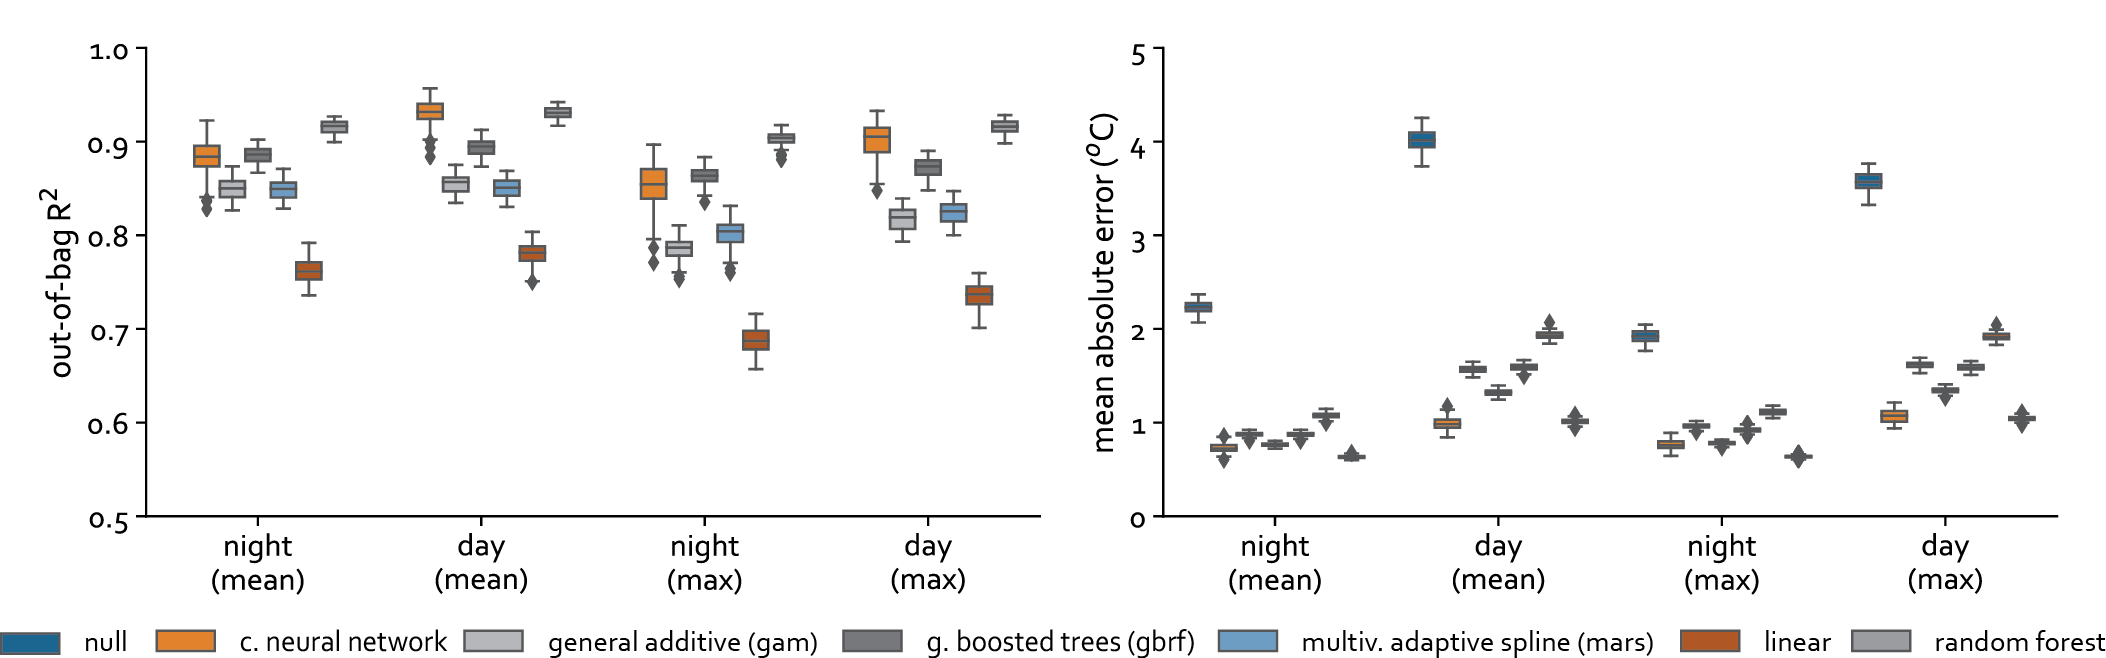
\includegraphics[width=\linewidth]{fig/report/holdout_100.png}
    \caption[Holdout cross-validation results at 100-meter resolution]{
    Holdout cross-validation results at 100-meter resolution.
    The out-of-bag (OOB) R$^2$ and mean absolute error (MAE) of the models from a 100-fold holdout cross-validation. 
    The models were trained on 80\% of the data and tested on the unseen 20\%.
    When selecting data for the training and testing sets, spatial subsets were used to account for spatial similarities. 
    OOB R$^2$ can vary between $(-\infty, 1)$, where better models have a value near 1. 
    Good models have MAE near 0.
    }
    \label{fig:holdout_100}
\end{figure*}

\subsection{Variable importance and influence}
Our objective with this study is to determine the influence and importance of various urban surface characteristics on land surface temperatures.
In this section we present results showing the importance and influence of the variables used in the statistical models.
However, in statistical modelling, one challenge to understanding influence and importance is decoupling variables that are often interrelated.
Failing to do this can result in confounding variables.
In Section 2.4, we describe how we select variables to reduce this by removing those that are correlated and multicollinear.
In doing so, we found that in this dataset tree canopy is 100\% negatively correlated with impervious surfaces (Figure \ref{fig:imp_tree}).
Therefore, we do not include \% impervious surface as a variable in the models, but it means that the terms tree canopy and pervious surface are equivalent when used in relation to the variables in the statistical models.

\begin{figure*}
    \begin{center}
    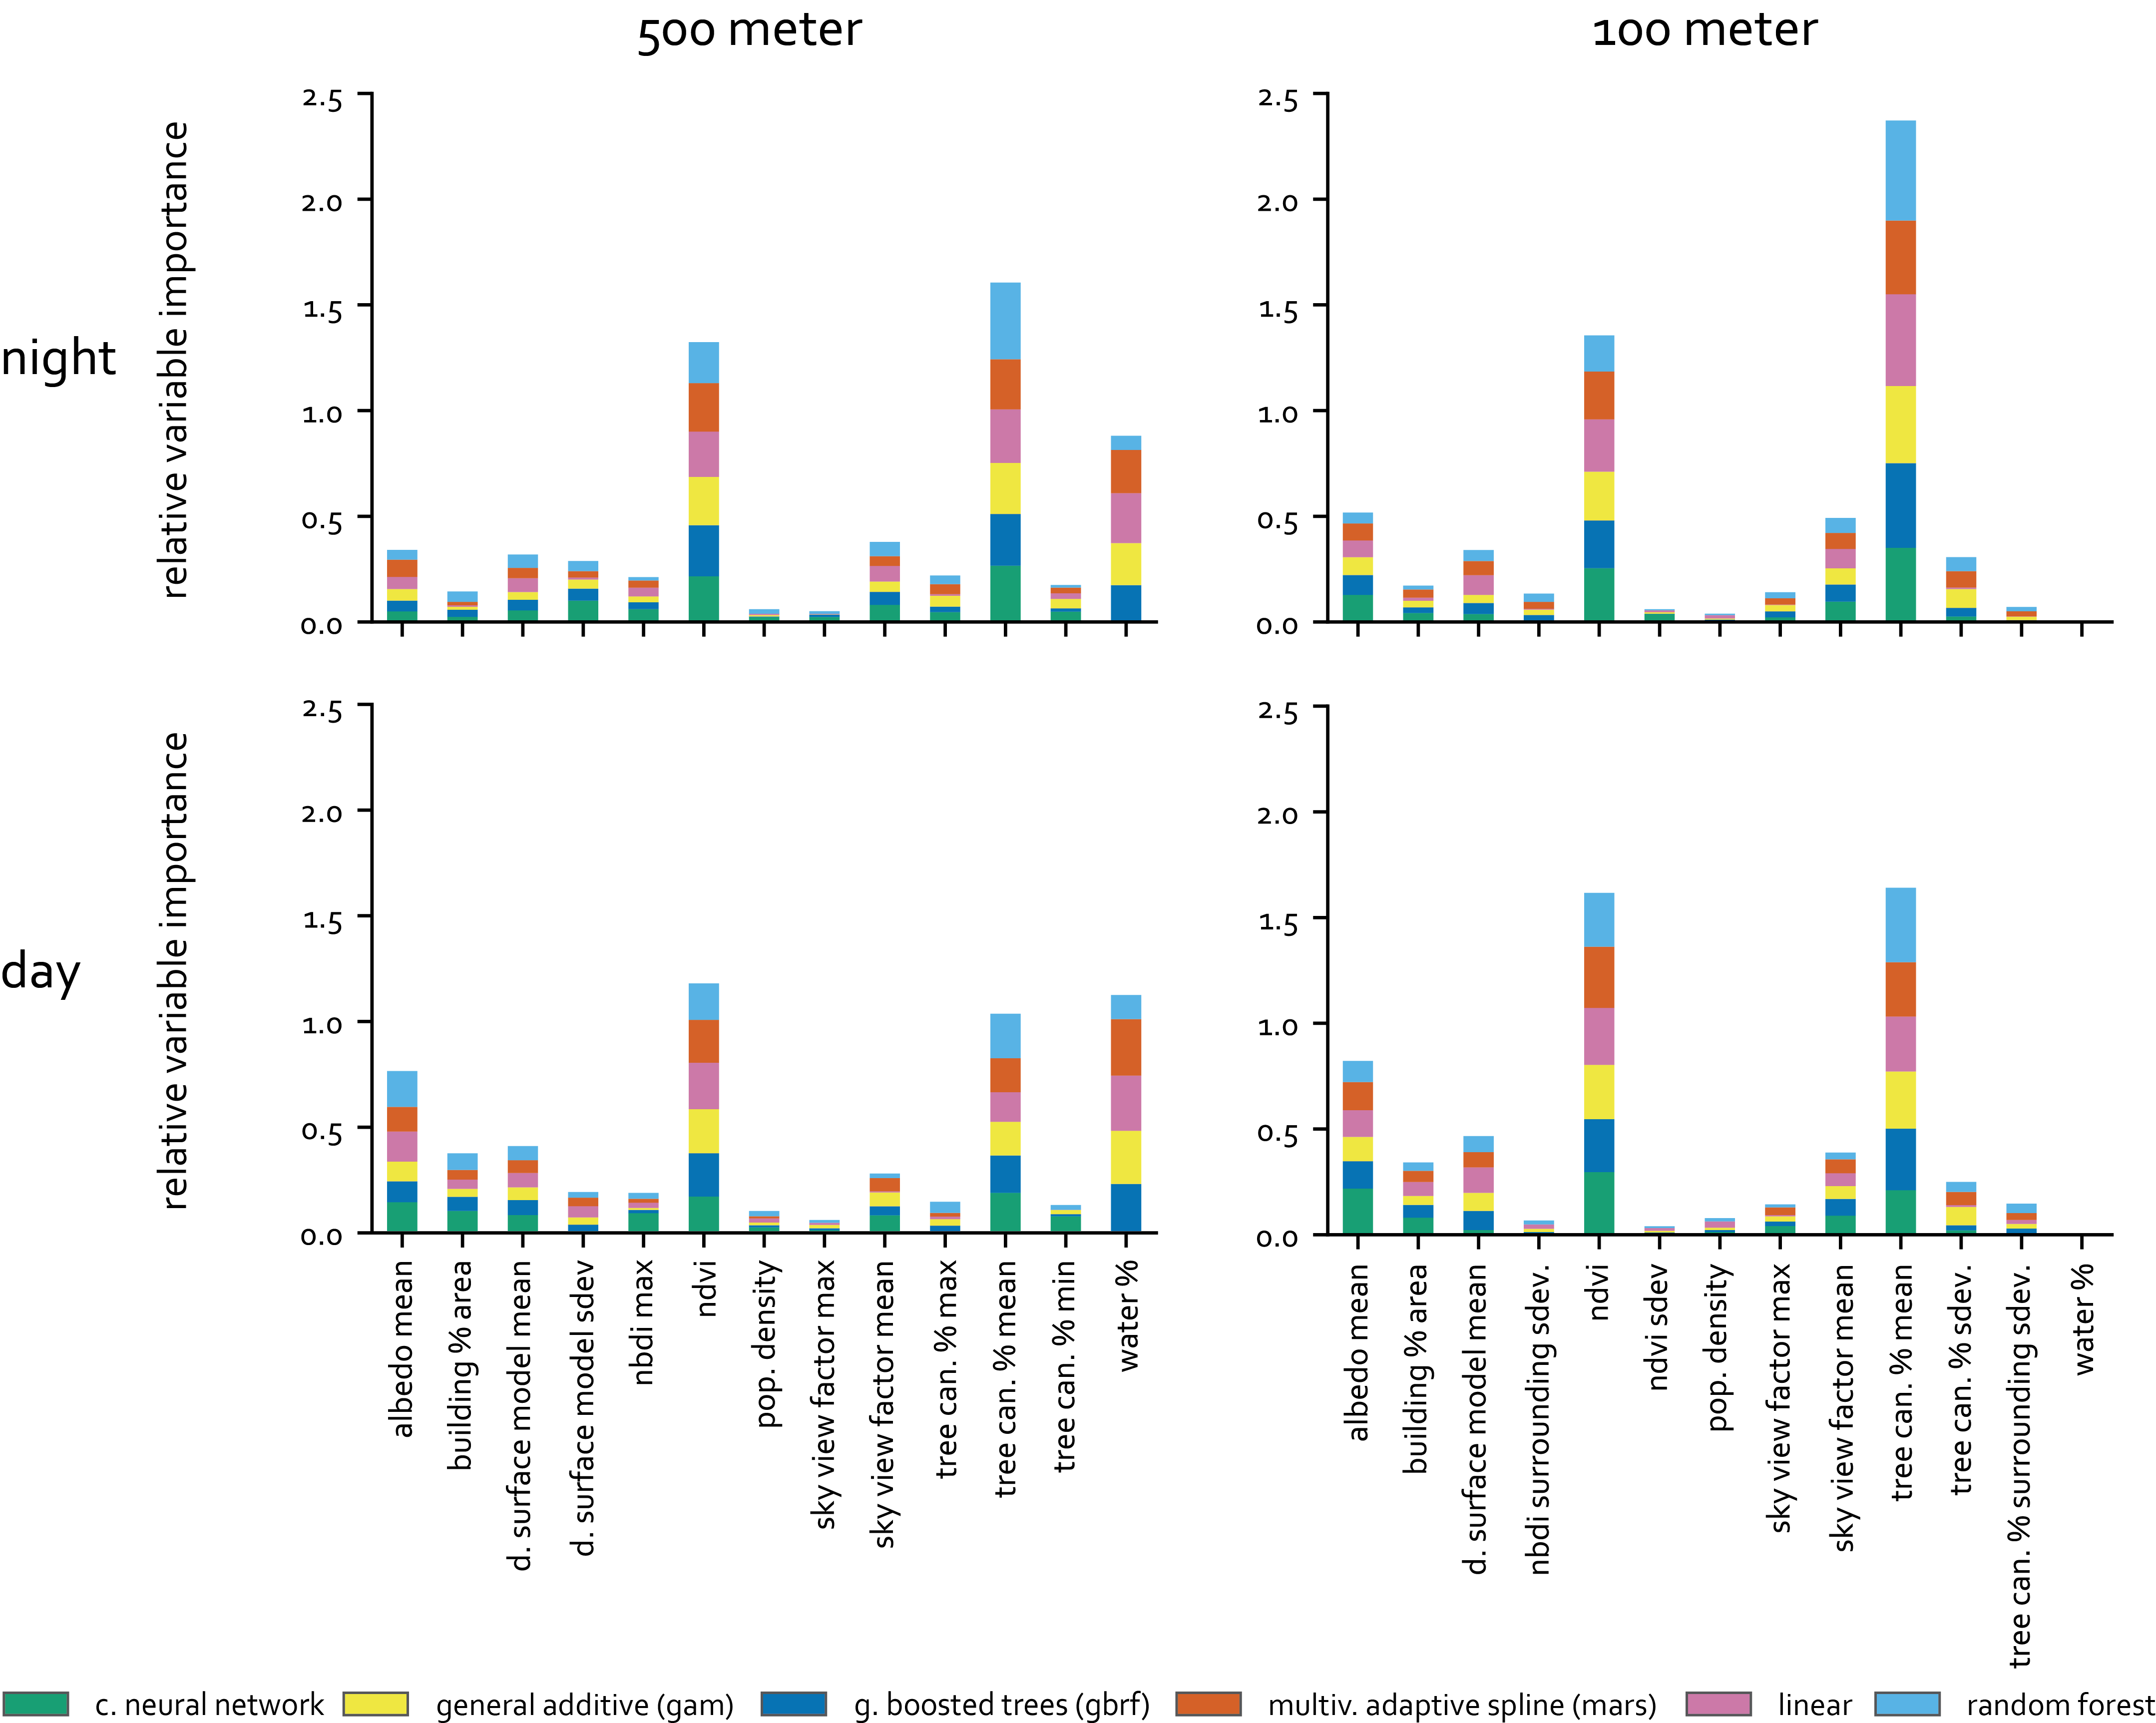
\includegraphics[width=\linewidth]{fig/report/importance_stacked.png}
    \caption[The relative importance of variables on land surface temperature]{
    The relative importance of variables on land surface temperature. 
    The variable influence, measured by swing, shows the relative importance of each urban characteristic on land surface temperature for each model. These results are then weighted by the each model's R$^2$ value and stacked to show which variables, across all of the models, have the largest influence on land surface temperature.
    
    Both 100 and 500 meter resolutions are shown to demonstrate the agreement and disparity across the spatial scales.
    }
    \label{fig:importance_stack}
    \end{center}
\end{figure*}

\begin{figure*}
    \centering
    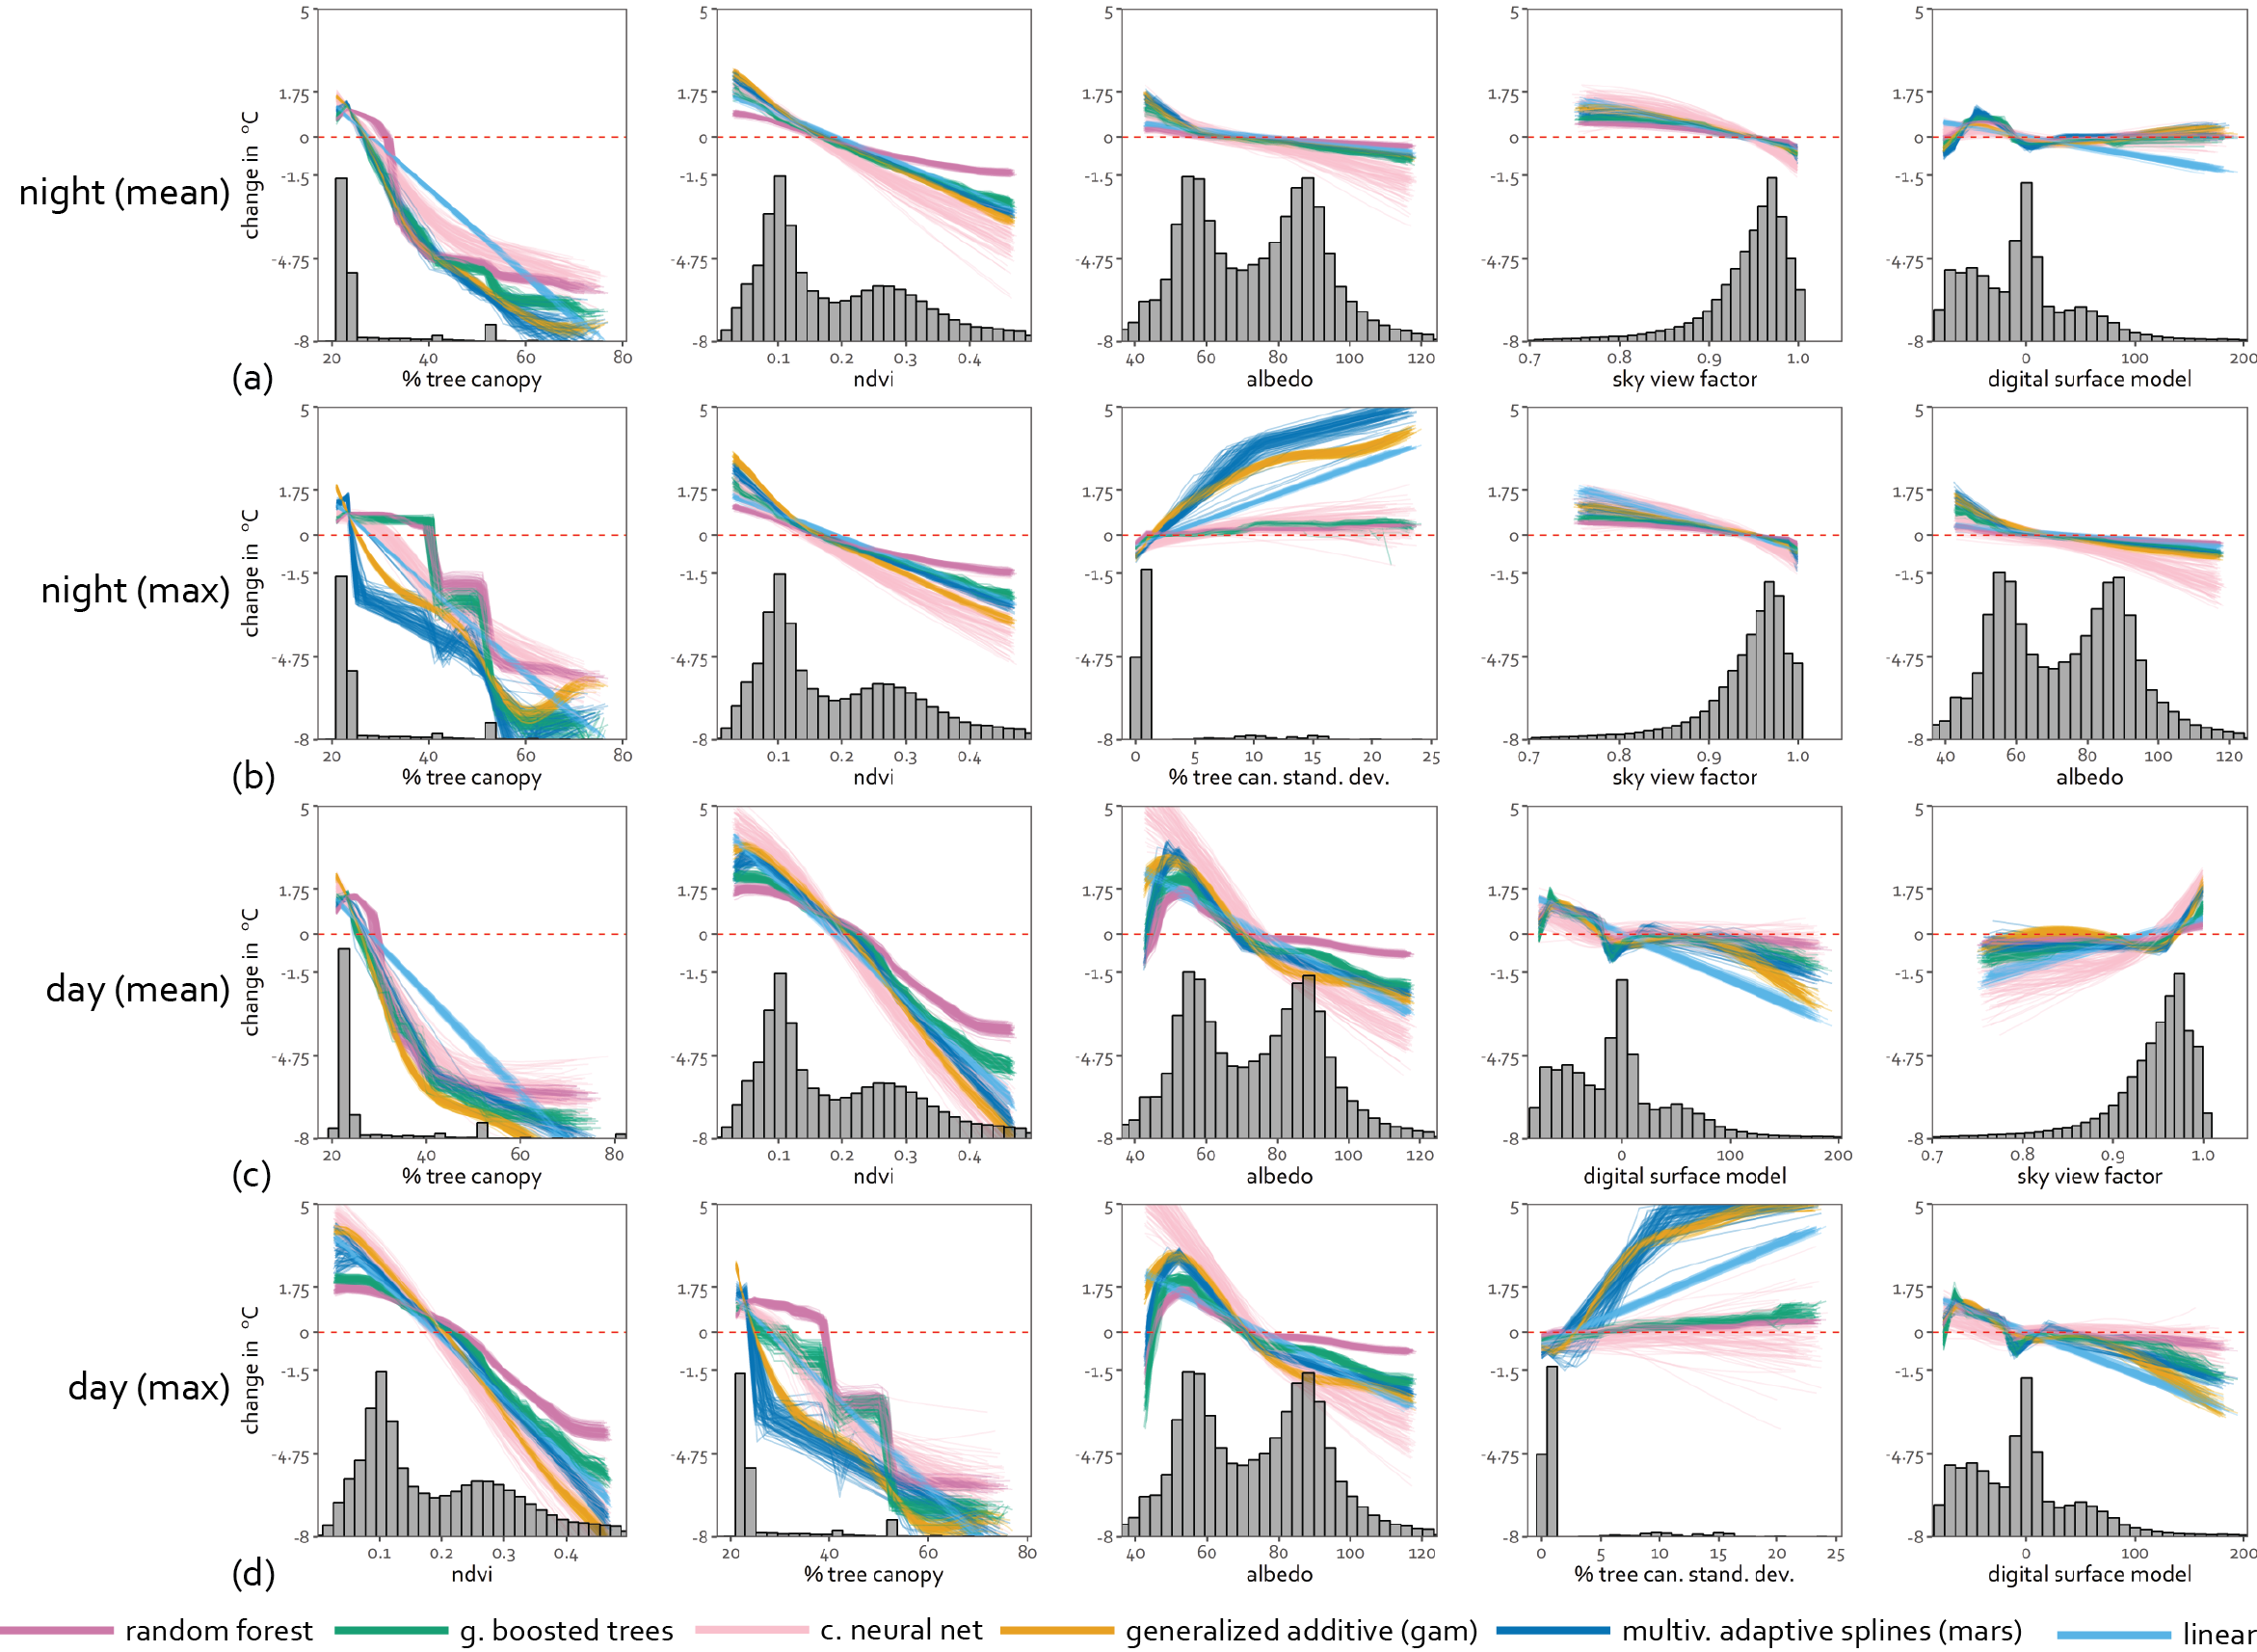
\includegraphics[width=\linewidth]{fig/report/pdp_100.png}
    \caption[Partial dependence plots for LST at 100-meter resolution]{
    Partial dependence plots for LST at 100-meter resolution.
    Partial dependence plots show how the land surface temperature ($^oC$, y axis) changes with each urban characteristic as the other variables are held at their average (mean) value. 
    The left hand side shows the effect each variable has on the (a) mean land surface temperature (LST) during the night, (b) maximum LST during the night, (c) mean LST during the day, (d) maximum LST during the day. 
    Each of the models are shown and this indicates the model uncertainty in the relationships.
    There are multiple lines for each model based on bootstrap samples of the data, which indicates the data uncertainty.
    The histograms on the $x$-axis show the distribution of the observed data.
    This is for the 500-meter resolution.
    }
    \label{fig:pdp_100}
\end{figure*}

Figure \ref{fig:importance_stack} presents the relative importance for each of the urban characteristics included in the models.
This stacked bar graph shows the cumulative importance of each variable to each statistical model, and is weighted by the R$^2$ of each statistical model.
The unweighted results are shown in Figures \ref{fig:importance_100} and \ref{fig:importance_500}.
The most important characteristics during the night are tree canopy cover and greenness (NDVI).
The sky view factor and the elevation (digital surface model) also appear important. 
The albedo is found to be important when assessing the 100-meter data, while the \% area covered in water is important with the 500-meter data; 
This is likely due to 98\% of the cells at 100m resolution having 0\% water, so the effect on the data set is negligible.
The important urban characteristics are consistent for both the mean and maximum temperature during the night.

The characteristics are also relatively consistent between night and day and between the models. 
Tree canopy and NDVI remain among the most important factors, however in the 500-meter dataset water is found to be the most important.
The importance of albedo is much higher for these daytime models than those using nighttime LST.

The minor association between albedo and nighttime temperatures is surprising given that darker surfaces store heat during the day that is released during the night \citep{Voogt2003-mm, Zhou2014-wc}.
However, this may be due to the nature of the remotely sensed data which captures the `seen' surface of the urban environment \citep{Roth1989-jj}; 
this `seen' surface is what is visible from a bird's eye view of the city, including roof-tops, tree-tops, roads, and open flat areas \citep{Roth1989-jj}.
These areas are likely more exposed to air flow and may store less heat than other surfaces within the city.
The relatively small reported importance of the sky view factor may also be due to the data sampled by satellites.
These data will likely under-sample vertical surfaces and those under canopies \citep{Roth1989-jj, Arnfield2003-gn} and so this must be considered when analyzing the results \citep{Roth1989-jj}.

Variable influence is shown in Figures \ref{fig:pdp_100}-\ref{fig:pdp_2dday_100} and \ref{fig:pdp_500}-\ref{fig:pdp_2dday_500}. 
These are the partial dependence plots and show how the surface temperature changes, on average, with the change to that variable.
Figures \ref{fig:pdp_100} and \ref{fig:pdp_500} show how LST changes with changes to one covariate.
Figures \ref{fig:pdp_2dnight_100}, \ref{fig:pdp_2dday_100}, \ref{fig:pdp_2dnight_500}, and \ref{fig:pdp_2dday_500} show the changes in LST as two variables change.

\textit{Vegetation and impervious surfaces}. 
During the day, increasing impervious surfaces and decreasing vegetation will increase sensible heat flux and lower latent heat flux \citep{Voogt2003-mm, Peng2012-iy, Zhou2014-wc}.
During the night, this process is thought to be less important because while latent and sensible heat are dominant during the day, ground heat flux dominates at night \citep{Zhou2014-wc, Voogt2003-mm}.
Indeed, because transpiration does not occur at night, vegetation's effect on night temperatures is debated. 
Our variable importance plots show that \% tree canopy (recall that in this study this is equivalent to \% pervious surface) is the most important factor on surface temperature during the night.
This is corroborated by the partial dependence plots.
Figure \ref{fig:pdp_100} shows that as tree canopy increases, the surface temperature decreases (a decrease in up to 10$^oC$ as the percentage area of trees or other pervious surface increases).
There is strong agreement between the statistical models, although the nonlinear models indicate a sharp decline in the average (mean) temperature with an initial tree canopy cover and suggest that this effect (the lines' gradients) weakens with a higher tree canopy cover.
This weakening may also be related to the sparser data at the upper tail of the dataset, and this is indicated by the wider uncertainty.

NDVI, a measure of the surface's greenness, was reported to be the next most important factor on land surface temperature. 
Given the conflation between tree canopy cover and impervious surfaces, NDVI can help to distinguish between vegetated surfaces and other pervious surfaces.
The relationship between NDVI and LST is surprisingly linear (Figure \ref{fig:pdp_100}), which clearly indicates that the greener a surface, the cooler it is.

The two-dimensional partial dependence plots (Figure \ref{fig:pdp_2dnight_100}) enable us to further evaluate this relationship.
By considering the joint effect of NDVI and tree canopy we can infer whether the influence on temperature is due to vegetation or simply pervious surfaces. 
The greener (higher NDVI) and more pervious (higher \% tree canopy cover) a surface is, the cooler it is during the night. 
The total change here is also approximately 7.5$^oC$, which is a considerable amount given these two-dimensional partial dependence are calculated using the random forest model, which is the least sensitive of the five models (as seen in Figure \ref{fig:pdp_100}).
These results do not support existing conclusions that vegetation has no effect on nighttime LST \citep{Peng2012-iy, Zhou2014-wc};
although much of the reduction in temperature could be due to the perviousness of the surface, lowered temperatures appear to be associated with the greenness (NDVI) of a surface during the night.

During the day, we again see that vegetation and impervious surfaces are associated with the greatest reduction in land surface temperature, with approximately 15$^oC$ change (Figure \ref{fig:pdp_2dday_100}: ndvi vs. \% tree canopy). 
This daytime result is consistent with expectation \citep{Chun2017-mm, Peng2018-cp, Wang2019-tree,Zhou2014-wc, Chun2018-so}.

An ongoing research step is determining the ideal vegetated and pervious surface.
This is because there is significant diversity in the cooling effectiveness of different types of green coverage \citep{Saaroni2018-ct}. 
For example, the effect of street trees can be highly localized \citep{Coutts2016-og}, while some types of trees cope with heat better than others \citep{Leuzinger2010-si}. 
Additionally, there are trade-offs with irrigation on vegetated surfaces \citep{Gober2009-im}.
There is also likely significant differences between tree canopy vs ground-level vegetation that cannot easily be discerned from remotely sensed studies given the data limitations.
However, these results show the importance of vegetated and pervious surfaces at a larger scale, which should motivate further investigation into the finer urban scales.
Understanding these differences will guide planning measures in urban spaces.

\textit{Water}.
Water is widely expected to decrease the LST during the day \citep{Wicki2017-fv, Zhou2018-iy, Wang2019-water}, but some claim that it may also increase LST during the night \citep{Chun2017-mm}.
The rationale is that water releases heat during the night, resulting in elevated nighttime temperature \citep{Chun2017-mm}.
This behavior may change depending on the water body’s characteristics, the season, and location.
Our findings, however, show that, during the summer months, water reduces the LST during both the day and night (Figure \ref{fig:pdp_500}).
Although these results are not supported at the 100-meter resolution because 98\% of the data at the 100-meter level has zero percentage water.
At the 500-meter resolution, we see that the presence of water can decrease LST between 1.5 and 8$^oC$ during the night and by substantially more during the day (Figure \ref{fig:pdp_500}).
At the 500m scale this is likely referring to larger water bodies, however the depth and other water characteristics are not evaluated.

\textit{Urbanization}.
Urbanization can lead to heat storage in roads and buildings \citep{Zhou2014-wc, Voogt2003-mm}. 
We discussed the role of impervious surfaces, alongside the effect of vegetation, but the statistical models also analyzed the influence of albedo, the percentage area of building, the NDBI (built-up index), and the sky view factor (a measure of the urban canyon effect).
The results for albedo are surprisingly low (Figure \ref{fig:importance_stack}): 
At night it is vastly less important relative to the vegetation and pervious factors, during the day it has more of an influence.
At both the night and day times sampled, albedo has a negative effect on temperature (Figure \ref{fig:pdp_100}).
During the day, this is most pronounced, and more reflective surfaces appear to be more than 5$^o$C cooler than others.
There is the potential that the effects of albedo on temperature are potentially confounded as both vegetation and impervious surfaces can have low albedo.
This highlights the utility of statistical models that can evaluate the effect of multiple variables.
We can investigate this further using the 2D partial dependence (Figures \ref{fig:pdp_2dnight_100} and \ref{fig:pdp_2dday_100}). 
Consider the plot showing the \% tree canopy vs albedo: the highest temperature occurs when there are dark impervious surfaces (bottom left).
While increasing the tree canopy (or, in this case, perviousness of the surface) will reduce temperature, we also see that the lowest temperature is with high ``\% tree canopy'' and high albedo.
Additionally, we see that albedo has little affect at night, although the highest temperature does occur when there is high acreage of building footprint with low albedo (Figure \ref{fig:pdp_2dnight_100}a).
%  increasing the reflectance decreases the temperature (Figure \ref{fig:pdp_100}).
During the day, albedo has a greater influence: the highest temperatures are observed when there is significant building area and low albedo (Figure \ref{fig:pdp_2dday_100}a), as well as high impervious area and low albedo (Figure \ref{fig:pdp_2dday_100}b).
Our results show that albedo decreases LST during the day, as expected \cite{Oke2017-or}.
However, in contrast to existing studies \citep{Peng2012-iy, Zhou2014-wc}, we find no strong association between albedo and surface temperature during the night.

The built-up index (NDBI), \% building area, and digital surface elevation model also had relatively minor associations with LST.
The elevation (non-built-up) variable was excluded because it was found to be collinear with other variables; the digital surface elevation model was included and represents the elevation including buildings and vegetation.
However, this elevation only appears to have minor associations with land surface temperature (Figure \ref{fig:pdp_100} \& \ref{fig:pdp_500}).
The building area had no effect during the night and minorly increased temperature during the day (Figure \ref{fig:importance_100}).
Maximum NDBI appears to have a slight positive association with maximum daytime LST (Figure \ref{fig:pdp_500}), but this effect is not observed at the 100m resolution.
This minor-to-negligible relationship is surprising given that NDBI has been reported as among the most important urban characteristics during the day \citep{Peng2018-cp}.
However, the discrepancy may be due to \% impervious surface area being incorporated already with the \% tree canopy data.

The canyon effect is also often attributed with causing warmer temperatures \citep{Chun2017-mm}, in particular, warmer air temperatures due to the urban canopy layer \cite{Oke1988-re}.
While there was high uncertainty in the models, it appears that during the night, the temperatures decrease as the sky view factor increased (Figure \ref{fig:pdp_100}a,b).
This is due to heat being captured within the canyons (areas with low sky view factors) due to changes in the air flow and energy exchange \cite{Oke1982-px} and, conversely, more exposed areas with high sky view factors will release their heat.
This is shown in the two-dimensional partial dependence plot (Figure \ref{fig:pdp_2dnight_100}e) where the higher temperatures are observed when there is high \% building area and low sky view factor.
It follows that heat is being captured in the canyons. 
However, compared to the other urban characteristics this has a lesser affect, changing the temperature by approximately 1.5$^o$C.
The effect of the sky view factor during the day is low-to-indiscernible (Figures \ref{fig:importance_100} and \ref{fig:pdp_2dday_100}f), but suggests that there are higher temperatures when the sky view factor is high.
Given that the relationship between urban canyons and urban temperatures is well-studied and known to exist \cite{Arnfield2003-gn}, the indiscernible relationship found here may reflect the limitations of remotely sensed data to investigate this effect.
This is due to the satellite imagery over sampling surfaces that are `seen' and therefore will include a lower proportion of areas that are within canyons that are obstructed by the structures that create the canyon \cite{Roth1989-jj}.

\textit{Population density}.
We found that population density had no discernible effect during night or day (Figure \ref{fig:importance_100}).

\subsection{Result sensitivity}.
To assess the robustness of the results, we conduct the analysis again at the 500-meter resolution (\ref{ss:500_meter}).
The results are consistent.
Additionally, to ensure that the effects are consistent between cities, we construct the partial dependence plots for each city (\ref{ss:city}).
The partial dependence is similar to Figure \ref{fig:pdp_100}.
Therefore, the consistency between 100 and 500-meter lends confidence to these conclusions.

\begin{figure*}
    \centering
    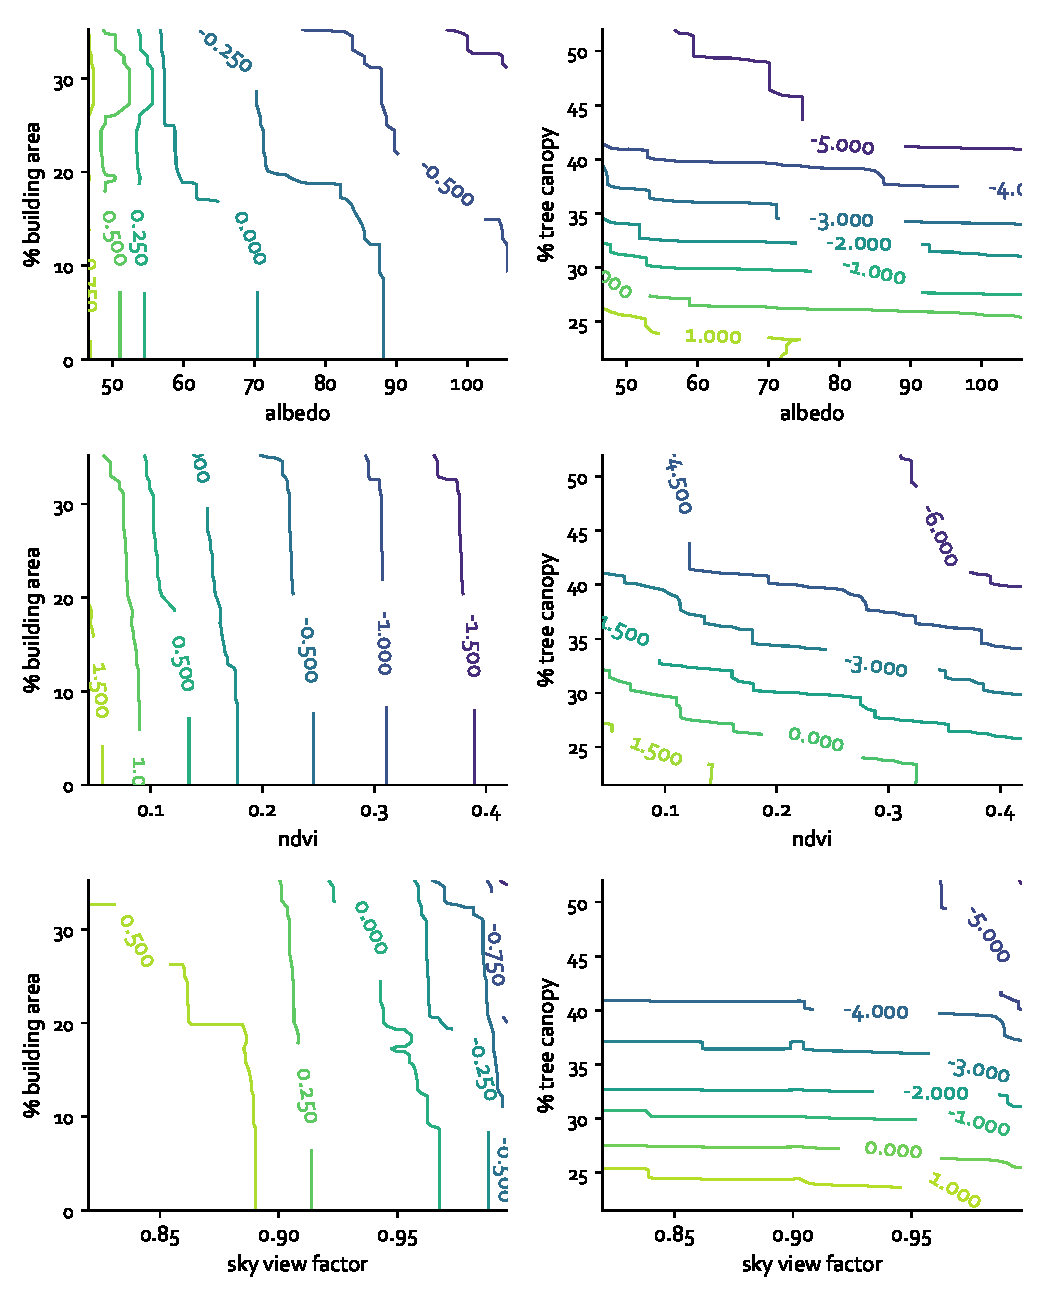
\includegraphics[width=\linewidth]{fig/report/pdp_2d_night_100.pdf}
    \caption{
    \textbf{Nighttime, mean}: A two-dimension partial dependence contour plot showing how the land surface temperature ($^oC$) at 100-meter resolution changes with the two variables shown on the $x$ and $y$ axes, while the remaining variables are held at their average value.
    This figure is the two-dimensional equivalent of Figure \ref{fig:pdp_100}, except with only the random forest model and without the uncertainty shown.
    }
    \label{fig:pdp_2dnight_100}
\end{figure*}


\begin{figure*}
    \centering
    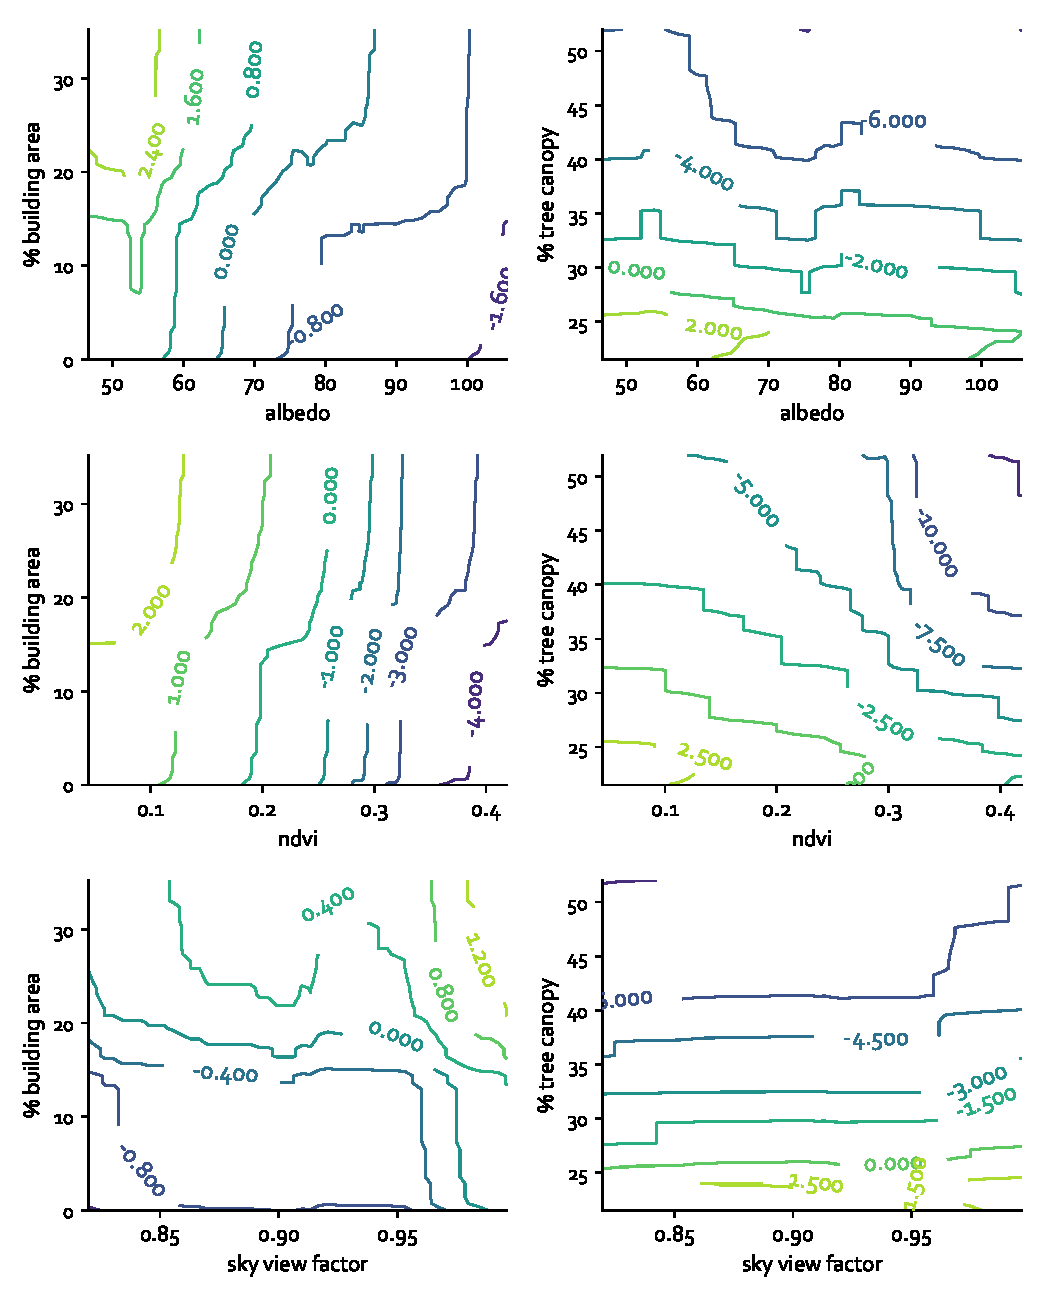
\includegraphics[width=\linewidth]{fig/report/pdp_2d_day_100.pdf}
    \caption{
    \textbf{Daytime, mean}: A two-dimension partial dependence contour plot showing how the land surface temperature ($^oC$) at 100-meter resolution changes with the pair of variables shown on the $x$ and $y$ axes, while the remaining variables are held at their average value.
    }
    \label{fig:pdp_2dday_100}
\end{figure*}

\section{Conclusion}
To assist planners tackling climate change, heat waves, and general high urban temperatures, we seek to determine how different urban characteristics are associated with land surface temperatures. 
The results strongly support initiatives for increasing green infrastructure in cities (e.g., \citep{Larsen2015-da, Meerow2017-xv}). 
We found that increasing vegetation and reducing impervious surface area had the greatest effect on surface temperature during both night and day, with the potential to reduce the temperature up to 10$^o$C.
While it is not surprising that vegetation and imperviousness are related to surface temperatures, this study is the first to quantify them for Landsat-resolution nighttime temperature estimates. 
These results are also useful for corroborating this relationship, because in complex urban environments it is far from clear that the anticipated behaviour would eventuate; for example, in the case of urban vegetation at night, much of the urban vegetation exists in water stressed environments that limit evaporative cooling, and so the mechanics and magnitude of the vegetation's effect on nighttime temperature is far from clear.
We also see strong evidence for blue space and increasing the area of water, although there are various limitations with doing so in cities such as Phoenix.
We do note that this analysis is for land surface temperature, and not air temperature. 
The correlation between LST and air temperature is varied at intra-urban scales, and the magnitude of LST variability tends to be larger than that of air temperature.
Also, remotely sensed data has limitations in that it cannot capture a representative sample of the urban environment, instead it favors surfaces seen from a bird's eye view.
Nevertheless, remotely sensed LST is a highly relevant variable for analyses of the urban energy balance, and thus for studies of the urban heat island and ways to ameliorate it.

Our findings demonstrate that accurate prediction of land surface temperature using urban characteristics is possible.
This result opens opportunities for further detailed analysis into potential interventions.
Such interventions for mitigating high temperatures are naturally place-specific, and while these results have proven general to four different US cities, work is needed to understand questions such as which types of greenery are better than others \citep{Gober2009-im}.

This study also demonstrates the opportunities of modern statistical techniques and the ability to assess potentially nonlinear interactions and the interactions between multiple variables. 
While the linear model did not perform as well as the more complex models, it was largely in agreement with the other models regarding the influence of the urban characteristics on land surface temperature.
The major limitation with linear models in this analysis is therefore the assumption that the relationship between surface temperature and each of the variables is constant (i.e., it doesn't change with the size of the covariate or dependent on any thresholds or other factors).
Another advantage of the advanced statistical models is their ability to analyze the interaction between factors, which is far less nuanced when using a linear model.
For example, in this analysis we were able to examine and disentangle the influence of two, often covarying, variables such as vegetation and albedo, and vegetation and NDVI.
These limitations may be perfectly suitable for many analyses, but are necessary to be aware of and considered when more detailed analysis is required.

Rigorous statistical analysis can continue to answer on-going questions central to land surface temperature.
For example, our results support the suggestion that 3D variables (e.g. sky view factor) do not outperform 2D ones (e.g. \% tree canopy cover) \citep{Berger2017-lx}. 
However, due to sampling limitations of the remotely sensed data, we do not believe the 3D variables are unimportant.
Additionally, we find some discrepancies between the analyses at the two spatial scales (notably in the effect and importance of water); this sensitivity is something that further studies should be aware of.
Our analysis is also not causal inference; such an analysis would require controlled variables and urban spaces.
We instead aim to complement and inform existing understanding of the relationships by demonstrating how land surface temperature and the urban characteristics are associated.
This can be used to inform potential strategies for urban heat reduction, that is, if an association exists between two variables then we can evaluate the potential for causality based on understanding the physical mechanisms.

However, if no association exists or is in the opposite direction of proposed strategies for heat reduction, then such strategies need to be re-evaluated.
For example, our results assessing the relative effect of sky view factor (a measure of building density), population, built-up index, and \% building area do not support claims advocating to constrain floor area ratios \citep{Chun2017-mm}.
Such policy could lead to increased urban sprawl (low-density or single-use urban development characterized by poor accessibility and a lack of functional open-space \citep{Ewing2015-xj}).
Instead, our results show that reducing impervious area and increasing vegetation and greenness have a stronger association with lowered temperatures.
Such action could be achieved without constraining floor area ratios.
If a constraint is explored, an additional necessary study is to compare sprawling and dense cities, prior to taking steps to dissuade density. 
Now that 100-meter resolution nighttime data are available, as well as the increasing availability of lidar data, studies advocating creative interventions such as increasing the vertical and horizontal randomness of buildings, increasing the prevalence of green roofs \citep{Gago2013-ta, Kelbaugh2019-th}, or other urban planning strategies can quantitatively be explored.

This study into daytime and nighttime land surface temperature in four US cities has highlighted the importance of vegetation in our cities' mitigation options. 
It has also demonstrated the utility of leveraging advanced statistical analysis to study land surface temperature.
The results are robust to both data and model uncertainty and are general across the cities studied.
They suggest that vegetation and impervious surfaces are the most important urban characteristics associated with land surface temperature.
Increasing and decreasing these, respectively, is necessary for reducing high urban temperatures during both night and day.

% There are various bibliography styles available. You can select the style of your choice in the preamble of this document. These styles are Elsevier styles based on standard styles like Harvard and Vancouver. Please use Bib\TeX\ to generate your bibliography and include DOIs whenever available.

% Here are two sample references: \citep{Feynman1963118,Dirac1953888}.
\section*{Acknowledgements}
The work was funded by the US National Science Foundation's Grant SEES-1631409 and a University of Michigan Rackham PreDoctoral Fellowship. 
This support is gratefully acknowledged.

\section*{References}
\singlespacing

\bibliography{mybibfile.bib}

\newpage
\onecolumn
\appendix

\section{Data sources}
The data sources for the analysis are listed in Table \ref{tab:data}. The satellite imagery used is described in Table \ref{tab:satellite_meta}. All of the data was gridded as shown in Figure \ref{fig:map}.

\begin{table}[H]
\caption{The data sources for the LST analysis.}
\label{tab:data}
\fontsize{8}{11}\selectfont
\begin{tabu}to \textwidth{ X[l]  X[c]  X[c] X[c] X[l] X[l] }
\toprule
 Data Provider & Data Type & Data Date & Resolution & Description & Source \\
 \hline
U.S. Geological Survey  & Raster  & 2013-2017 & 100m &
    Landsat 8 day and night satellite imagery & \url{https://earthexplorer.usgs.gov/} \\
Microsoft  & Polygon  & 2018 & n/a & Building footprint polygons for the US &
    \url{https://github.com/Microsoft/USBuildingFootprints} \\
% Defense Meteorological Satellite Program  & Raster  & 2013 &
    % Stable nighttime light intensity & \url{https://www.ngdc.noaa.gov/eog/dmsp/downloadV4composites.html} \\
Multi-Resolution Land Characteristics Consortium  & Raster  & 2011 & 30m &
    Land cover & \url{https://www.mrlc.gov} \\
Multi-Resolution Land Characteristics Consortium  & Raster  & 2011 & 30m &
    Percent developed imperviousness & \url{https://viewer.nationalmap.gov} \\
Multi-Resolution Land Characteristics Consortium  & Raster  & 2011 & 30m &
    Percent tree canopy cover & \url{https://viewer.nationalmap.gov} \\
U.S. Geological Survey  & Raster  & 2015 & 10m & 1/3 arc-second elevation & 
    \url{https://nationalmap.gov/3DEP/3dep_prodserv.html} \\
U.S. National Oceanic and Atmospheric Administration  & Lidar  & 2014 & 1m (Detroit) - resolved to 6m & Point cloud of surface elevation &
    \url{https://coast.noaa.gov/htdata/lidar2_z/geoid12b/data/6377/} \\
IPUMS NHGIS  & Area Level  & 2010 & city block &
    Block-level population from the US census & \citep{nhgis}\\
\bottomrule
\end{tabu}

\end{table}

\begin{table}[H]
\caption{The date, time, and cloud cover information of the satellite images used for the remote sensing data. The night time images do not have percent cloud cover calculated in their metadata.}
\label{tab:satellite_meta}
\begin{tabular}{ll|lll}
          &       & date      & time  & \% cloud cover \\
          \hline
Baltimore & Day   & 07-Sep-17 & 11:46 & 11.6\%         \\
          &       & 22-Aug-17 & 11:46 & 0.7\%          \\
          &       & 18-May-17 & 11:45 & 20.3\%         \\
          &       & 18-Jul-16 & 11:46 & 11.5\%         \\
          &       & 02-Jul-16 & 11:46 & 1.4\%          \\
          & Night & 08-Sep-17 & 22:50 & -              \\
          &       & 05-Sep-16 & 22:50 & -              \\
          &       & 20-Aug-16 & 22:50 & -              \\
          &       & 04-Aug-16 & 22:50 & -              \\
Detroit   & Day   & 26-Sep-17 & 12:16 & 0.4\%          \\
          &       & 03-Jun-16 & 12:15 & 6.9\%          \\
          &       & 18-May-16 & 12:15 & 1.9\%          \\
          & Night & 04-Sep-17 & 23:16 & -              \\
          &       & 19-Aug-17 & 23:16 & -              \\
          &       & 18-Jul-17 & 23:15 & -              \\
          &       & 31-May-17 & 23:15 & -              \\
          &       & 15-May-17 & 23:15 & -              \\
Phoenix   & Day   & 01-Sep-17 & 11:03 & 0.0\%          \\
          &       & 16-Aug-17 & 11:03 & 0.0\%          \\
          &       & 15-Jul-17 & 11:03 & 2.2\%          \\
          &       & 29-Jun-17 & 11:03 & 0.0\%          \\
          &       & 13-Jun-17 & 11:03 & 0.0\%          \\
          & Night & 16-Sep-17 & 22:17 & -              \\
          &       & 31-Aug-17 & 22:17 & -              \\
          &       & 15-Aug-17 & 22:17 & -              \\
          &       & 28-Jun-17 & 22:17 & -              \\
          &       & 12-Jun-17 & 22:16 & -              \\
Portland  & Day   & 30-Jul-17 & 11:55 & 2.9\%          \\
          &       & 14-Jul-17 & 11:55 & 0.2\%          \\
          &       & 27-May-17 & 11:55 & 1.8\%          \\
          &       & 13-Sep-16 & 11:56 & 0.0\%          \\
          &       & 12-Aug-16 &       & 0.1\%          \\
          & Night & 28-Sep-17 & 22:45 & -              \\
          &       & 12-Sep-17 & 22:45 & -              \\
          &       & 27-Aug-17 & 22:45 & -              \\
          &       & 24-Jun-17 & 22:45 & -              \\
          &       & 23-May-17 & 22:45 & -             
\end{tabular}
\end{table}

\begin{figure*}
    \centering
    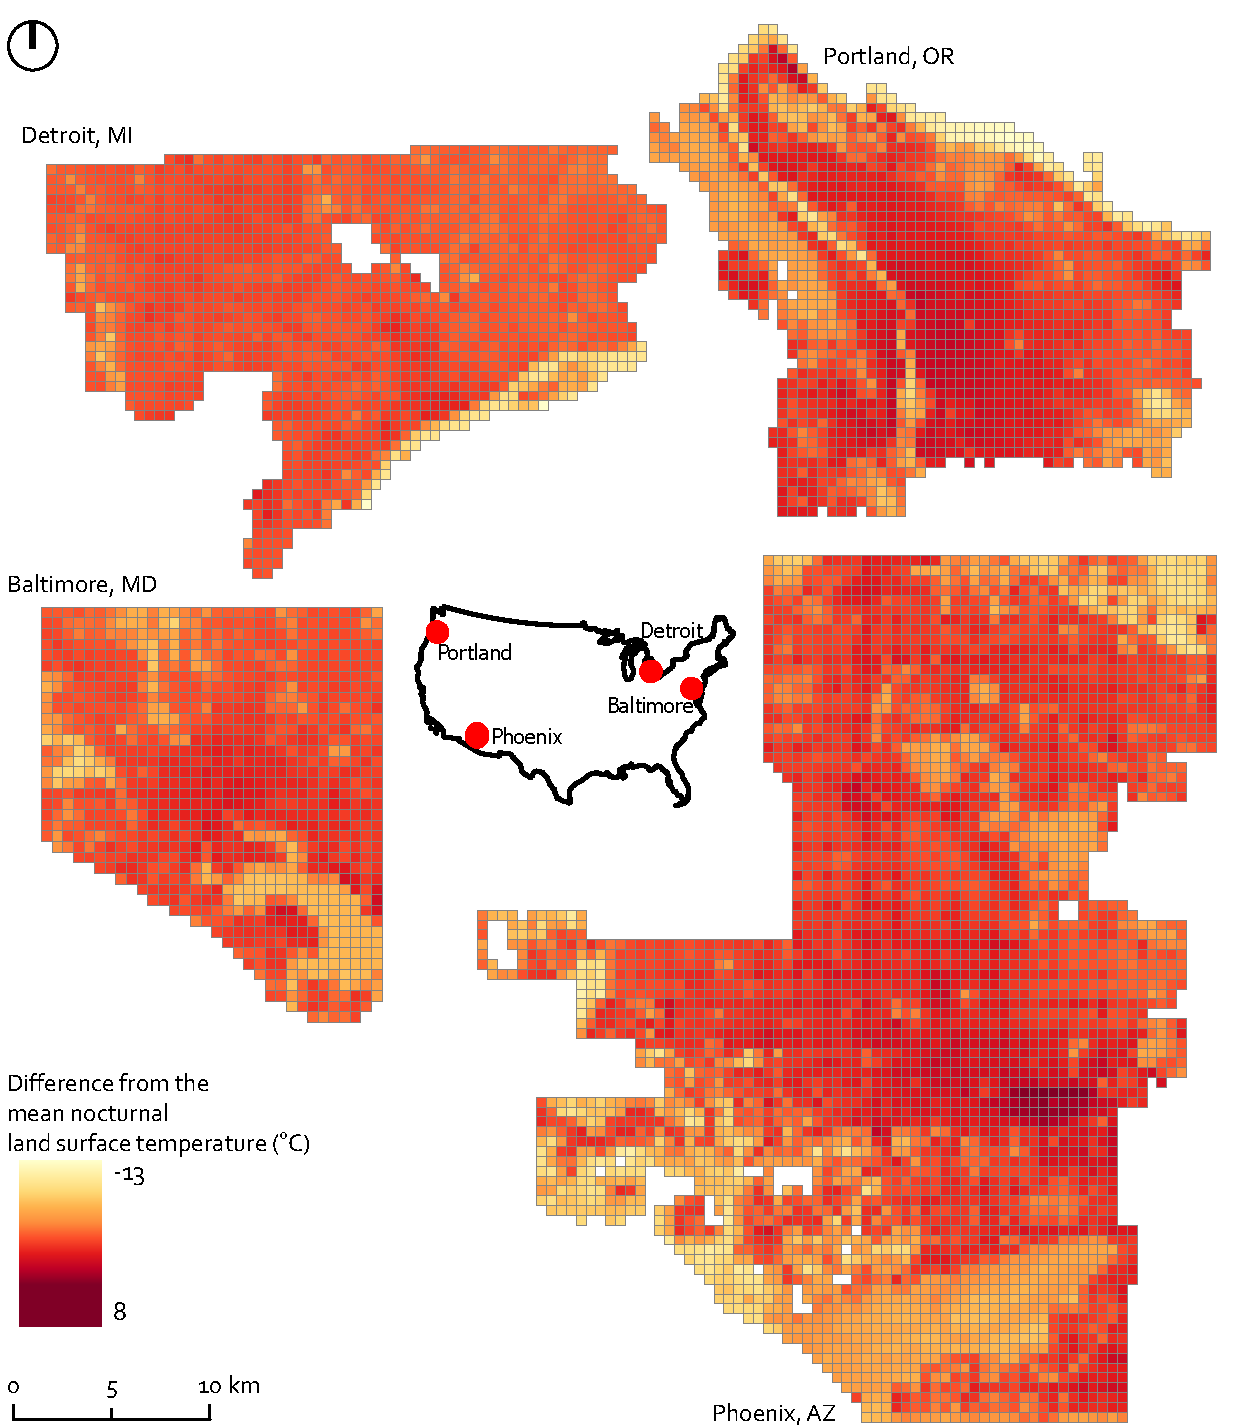
\includegraphics[width=\textwidth]{fig/report/map_nocturnal_lst.pdf}
    \caption[The nighttime land surface temperature in $^o$C, gridded into 500-meter cells]{The nighttime land surface temperature in $^o$C, gridded into 500-meter cells, for the cities studied. This is change from the mean (average) for each city.}
    \label{fig:map}
\end{figure*}


\newpage
\section{Code for the land surface temperature calculation}
\label{appendix:code}

This is an extract of the code provided in the GitHub repository: \url{https://github.com/tommlogan/land_surface_temperature}

\begin{lstlisting}[language=Python]


def calc_LST(info_satellite, meta_dict, source_city):
    '''
        Returns the land surface temperature (LST) based on satellite imagery
    '''
    # read in band 10 data
    image_b10 = gdal.Open(fn_b10)
    dn = image_b10.ReadAsArray()

    # conversion to TOA radiance
    TOA = calc_TOA(dn, meta_dict, 10)

    # emissivity correction
    emissivity = determine_emissivity(info_satellite, dn, source_city)

    # calculate the at-satellite brightness temperature
    temp_satellite = calc_satellite_temperature(TOA, meta_dict, emissivity)

    # atmospheric correction
    temp_surface = atmos_correction(temp_satellite, info_satellite, emissivity)


def calc_TOA(dn, meta_dict, band_number):
    '''
        Calculate the Top Atmosphere Spectral Radiance (TOAr) from Band 10 digital
        number (DN) data (also refered to as the Q_cal - quantized and
        calibrated standard product pixel value)
    '''

    TOAr = meta_dict['RADIANCE_MULT_BAND_{}'.format(band_number)] * dn + meta_dict['RADIANCE_ADD_BAND_{}'.format(band_number)]

    return(TOAr)


def calc_satellite_temperature(TOA, meta_dict, emissivity):
    '''
        Calculate the At-Satellite Brightness temperature
        First, need to calculate the emissivity from the land use
        Then convert
        Returns temperature in Kelvin
    '''
    # spectral radiance
    L_lam = TOA/emissivity

    # calculate the satellite brightness
    temp_satellite = meta_dict['K2_CONSTANT_BAND_10']/(np.log(1 + (meta_dict['K1_CONSTANT_BAND_10']/L_lam)))

    return temp_satellite


def atmos_correction(temp_satellite, info_satellite, emissivity):
    '''
        Using the mono-window algorithm (Qin et al., 2001, International Journal of Remote Sensing)
        make the atmospheric correction
        Returns land surface temperature in celsius
    '''

    # temparature from csv file
    temp_max = info_satellite['max_temp_celsius']
    # convert to Kelvin
    temp_max += 273.15

    # constants for the algorithm
    a_6 = -67.355351
    b_6 = 0.458606
    w = 1.6
    t_6 = 0.974290 - 0.08007*w
    # variables dependent on land cover (emissivity) and temperature
    c_6 = emissivity * t_6
    d_6 = (1 - t_6)*(1 + (1 - emissivity)*t_6)
    t_a = 16.0110 + 0.92621*temp_max

    # mono-window algorithm (Qin et al., 2001, page 3726)
    T = a_6*(1 - c_6 - d_6) + (b_6*(1 - c_6 - d_6) + c_6 + d_6)*temp_satellite - d_6*t_a
    temp_landsurface = T/c_6

    # converting to celsius
    temp_landsurface -= 273.15

    return temp_landsurface
\end{lstlisting}


\newpage
\section{Covariates included in models}


We select variables to include in the model based on the variance inflation factor (VIF). 
This approach removes variables that exhibit high multicollinearity, that is the variable can be predicted from a combination of other variables. 
It is important to remove variables with high multicollinearity in inferential studies because otherwise the variables may confound the effect of one another on the variables of interest.



\begin{table}[h]
% \small
% \fontsize{8}{11}\selectfont
\centering
\caption{Covariates included after accounting for multicollinearity.}
\label{tab:vif}
\begin{tabular}{p{0.23\linewidth} p{0.7\linewidth}}
\toprule
       \textbf{Resolution} & \textbf{Included variable} \\
\midrule
100-meter  & Albedo mean \\
& NDVI mean \\
& Sky view factor mean \\
& \% tree canopy stand. dev. spatial lag \\
& \% tree canopy stand. dev. \\
& NDBI stand. dev. spatial lag \\
& \% building area\\
& Sky view factor max \\
& \% tree canopy mean \\
& NDVI stand. dev. \\
& \% water area\\
& Digital surface model mean \\
& Population density mean\\
\hline
500-meter & NDVI mean \\ 
& Albedo mean \\
& Sky view factor mean \\
& Digital surface model stand. dev. \\
& \% building area\\
& \% tree canopy mean \\
& \% water area\\
& Sky view factor max \\
& NDBI max \\
& \% tree canopy max \\
& Population density mean\\
& Digital surface model mean \\
& \% tree canopy min \\
\bottomrule
\end{tabular}
\end{table}


\newpage
\section{Technical appendix: Convolutional neural network}
\label{ss:cnn}
\subsection{Overview}

Our CNN model was adapted from a U-Net architecture \citep{unet}. This architecture is commonly used for image segmentation: the input to a U-Net model is a 2D greyscale image, and the output is another 2D image with values representing the classification of each pixel. The novel property of a U-Net CNN is that the internal layers learn at various resampled resolutions of the input data, which makes the model good at learning phenomena that are driven at multiple scales.

Several modifications were made to adapt U-Net to a geospatial use-case, and are outlined below.


\subsection{Data preparation}

The gridded data for each city was treated as an image, with each pixel representing a 100m or 500m cell. Instead of having three channels (red, green, and blue) like a colour image, these images had one channel for each of the independent variables in the dataset. The target was a 2D single channel image of the same shape.

CNNs require all inputs to be the same shape, which isn't the case for our city domains. Each city image was therefore split into images of $32 \times 32$ pixels ($24 \times 24$ for the 500m resolution). Splitting the images up also gives more training samples to work with: each of the small square images is a training sample.

Because the city boundaries aren't square and contain holes, missing data are introduced when placing the data into square images. The missing data needs to be filled because neural networks have no built-in way to handle non-real numbers. A simple approach like replacing with the median for each variable would result in unrealistic abrupt spatial jumps near the city boundaries: these discontinuities would affect the convolution operations in the CNN which can rely on features such as edges and spatial variance. Instead, holes and concave boundaries were filled using linear interpolation, then edges were extended by setting missing-data corner pixels to the median value of each variable and performing linear interpolation. The progression of the missing data filling algorithm is shown in Figure~\ref{fig:cnn_missing_data}. The result is all-real images with smooth changes at the missing data boundaries.

\begin{figure*}[h]
    \centering
    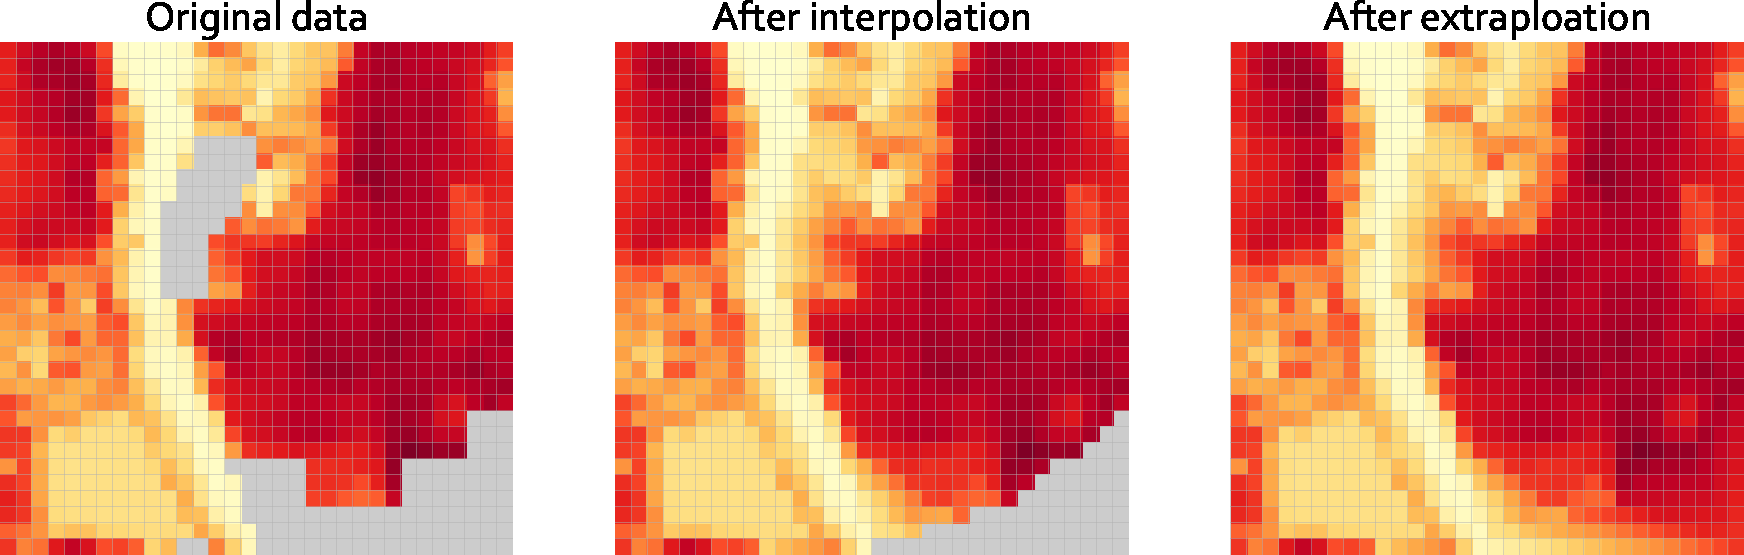
\includegraphics[width=\linewidth]{fig/report/cnn_data_prep.pdf}
    \caption{Handling of missing data for the CNN. The image shown is for a $32 \times 32$ cell section of mean day temperature for Portland at the 100m resolution.}
    \label{fig:cnn_missing_data}
\end{figure*}


\subsection{Model}

The model architecture is shown in Figure~\ref{fig:cnn_architecture}. It consists of multiple convolutional layers at both the input resolution and a 50\% downsampled resolution. Additionally, a skip connection concatenates the raw input data with one of final layers to reduce the depth between the input and output.

\begin{figure*}[h]
    \centering
    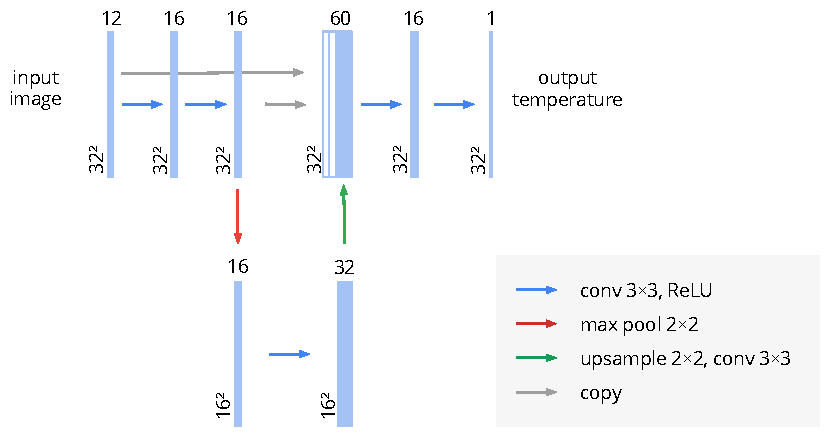
\includegraphics[width=\linewidth]{fig/report/cnn_architecture_cropped.pdf}
    \caption{CNN model architecture. Each layer shows the spatial dimensions (e.g., $32^2$) and the number of channels (e.g., 12). In the final {$32^2 \times 1$} layer, the ReLU layer is omitted.}
    \label{fig:cnn_architecture}
\end{figure*}

The size of the network is much smaller compared to the original U-Net in order to reduce overfitting due to our small dataset.

The final layer uses a linear activation function to enable regression. All other layers use ReLU activation, and dropout is applied after the contraction.

To prevent the CNN overfitting to the naively-imputed missing data, a masked loss function was used. The mean square error was greatly reduced for cells $i$ with missing data according to a mask $M$

\begin{align*}
    \mathrm{loss}_i &= M_i(y_i - \hat y _i) ^ 2\\
    M_i &= \begin{cases}
      0.01, & \text{if}\ y_i \mathrm{undefined} \\
      1, & \text{otherwise}
    \end{cases}
\end{align*}

This reduces the impact missing data has on the model weights, while leaving a small amount of gradient to avoid numerical issues with lack of convergence. The cells with missing data were excluded from any results presented.

The mask was also added to the input data as an additional channel.

\newpage
\section{Detailed variable importance results }
\label{ss:varimp}

The results shown in Figure \ref{fig:importance_stack} show the stacked variable importance where the relative variable importance for each model is weighted by the model's R$^2$ value. In these two figures the raw relative variable influence (calculated using swing) is presented. This allows for the differences between the models to be compared.

\begin{figure*}
    \begin{center}
    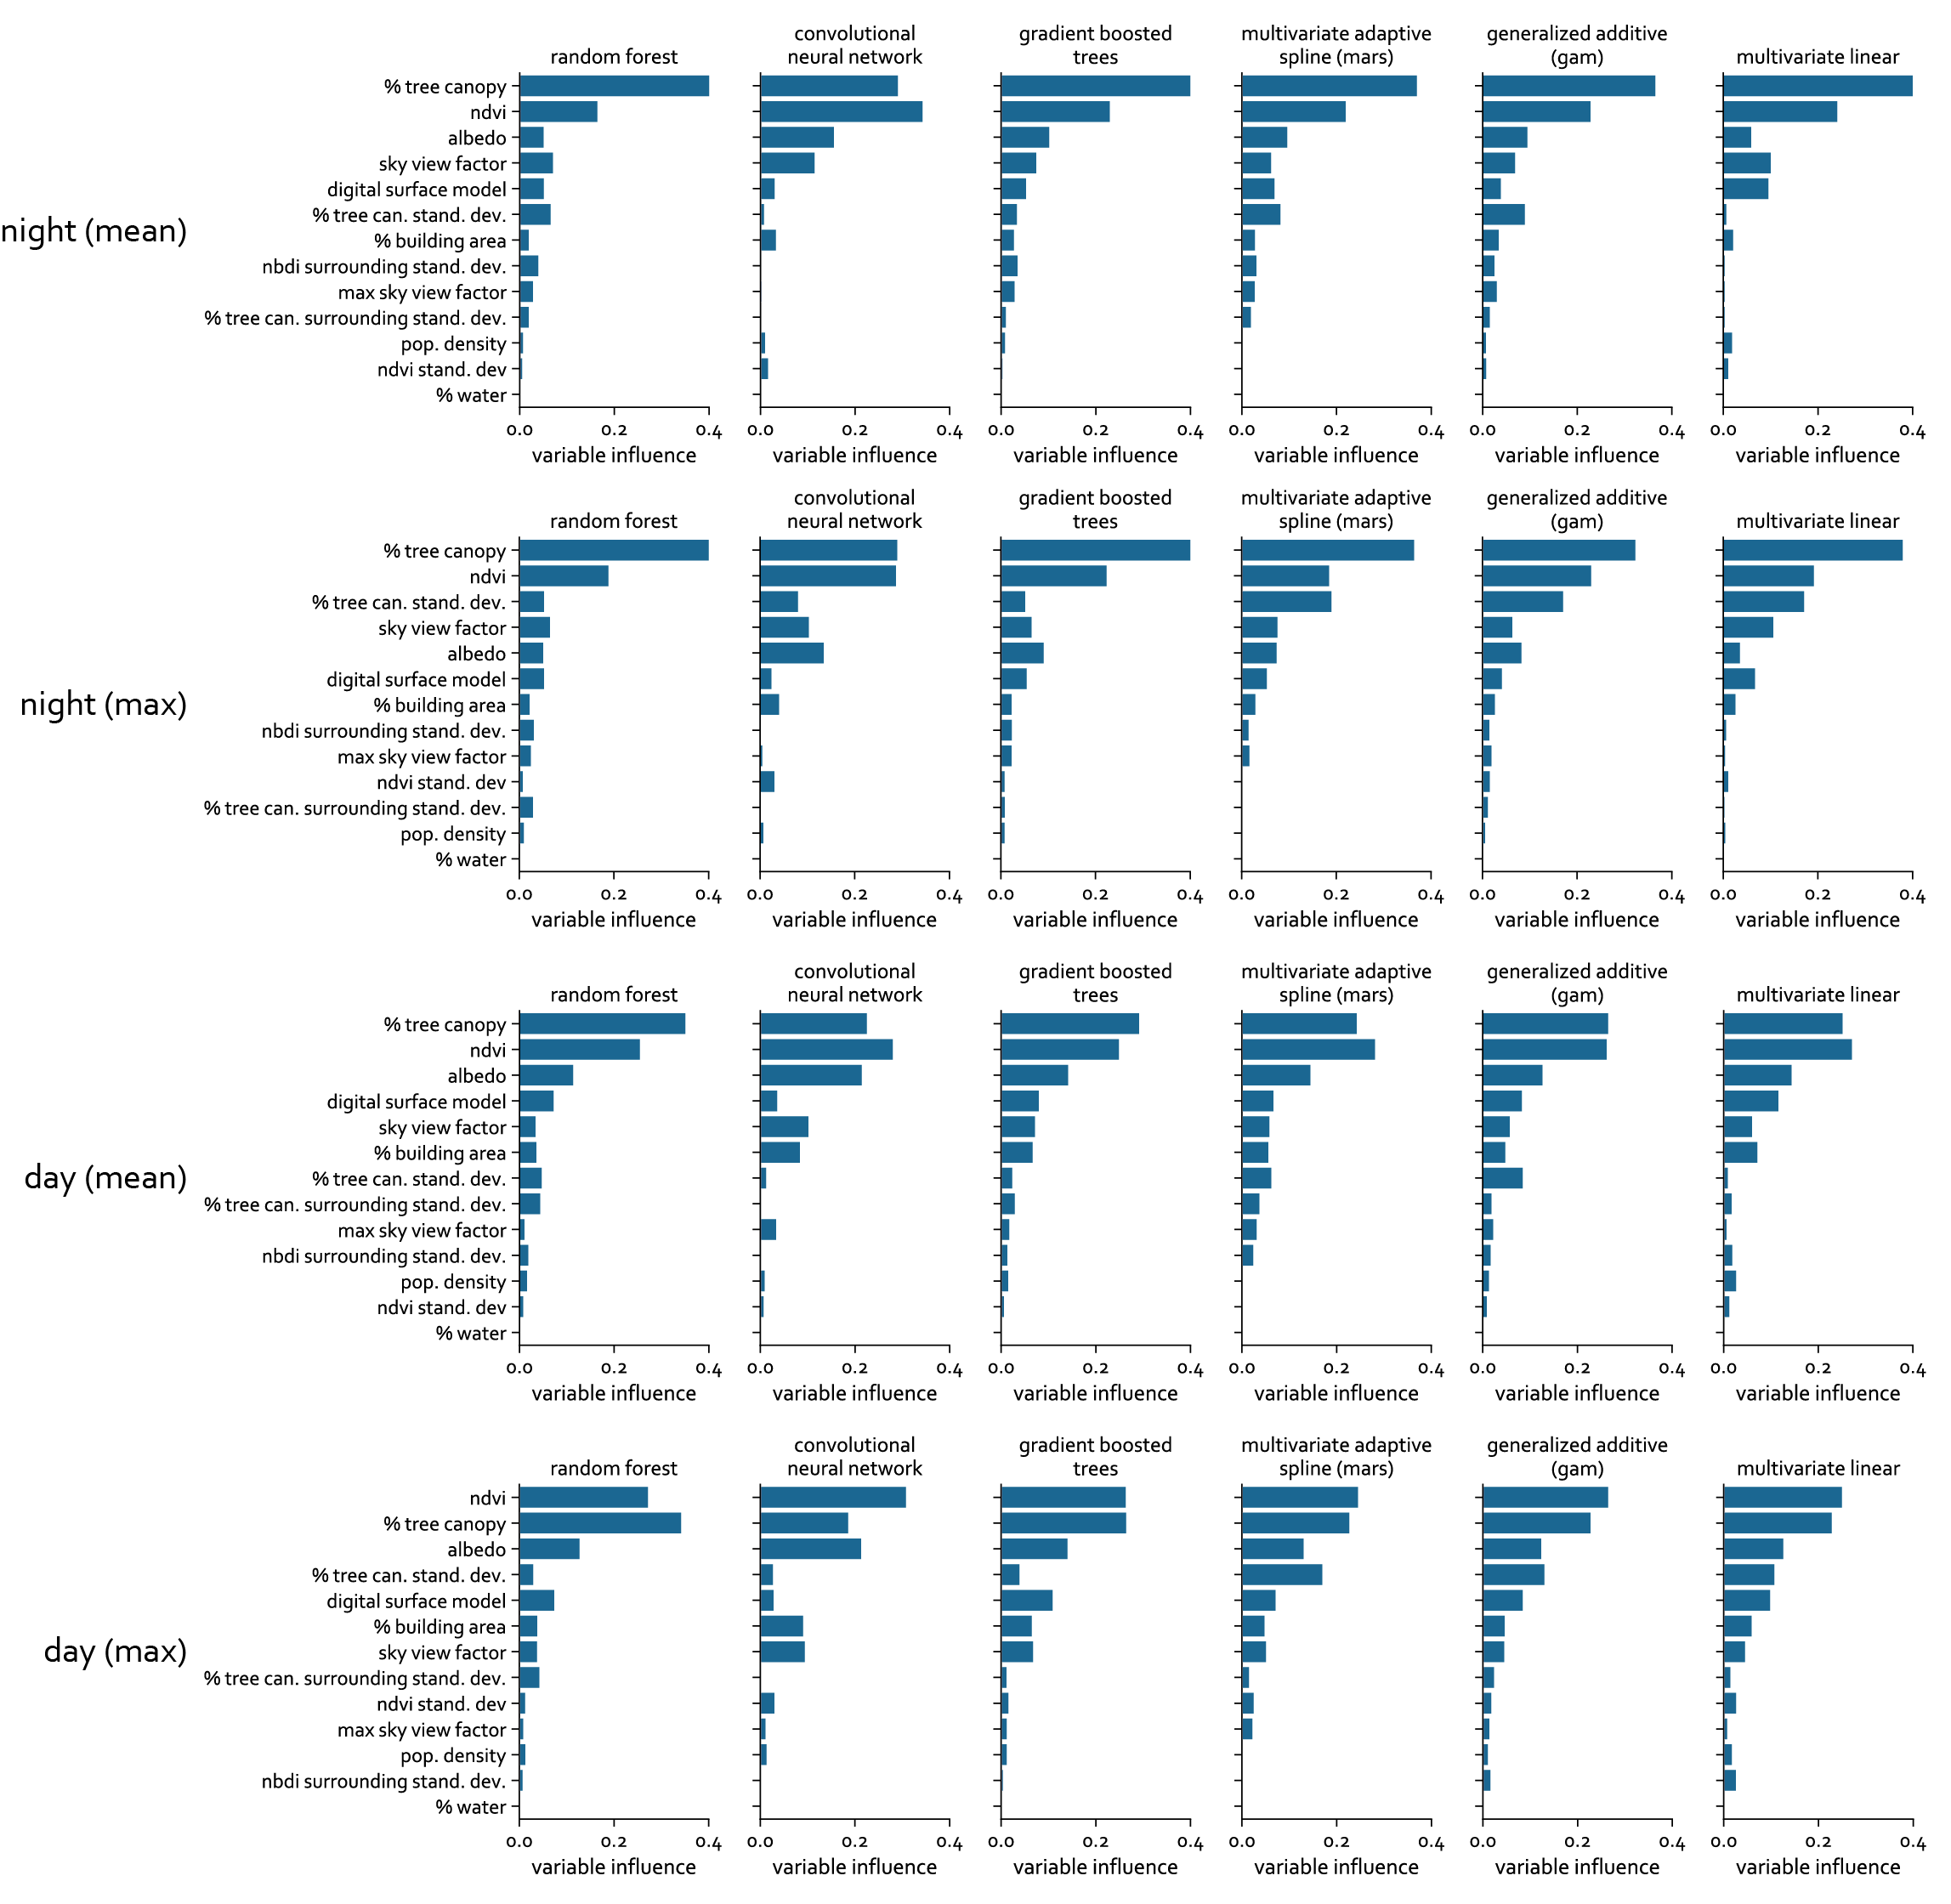
\includegraphics[width=\linewidth]{fig/report/importance_100.png}
    \caption[Variable influence on LST at 100-meter resolution]{
    Variable influence on LST at 100-meter resolution.
    The variable influence, measured by swing, shows the relative importance of each urban characteristic on land surface temperature.}
    \label{fig:importance_100}
    \end{center}
\end{figure*}


\begin{figure*}[h]
    \begin{center}
    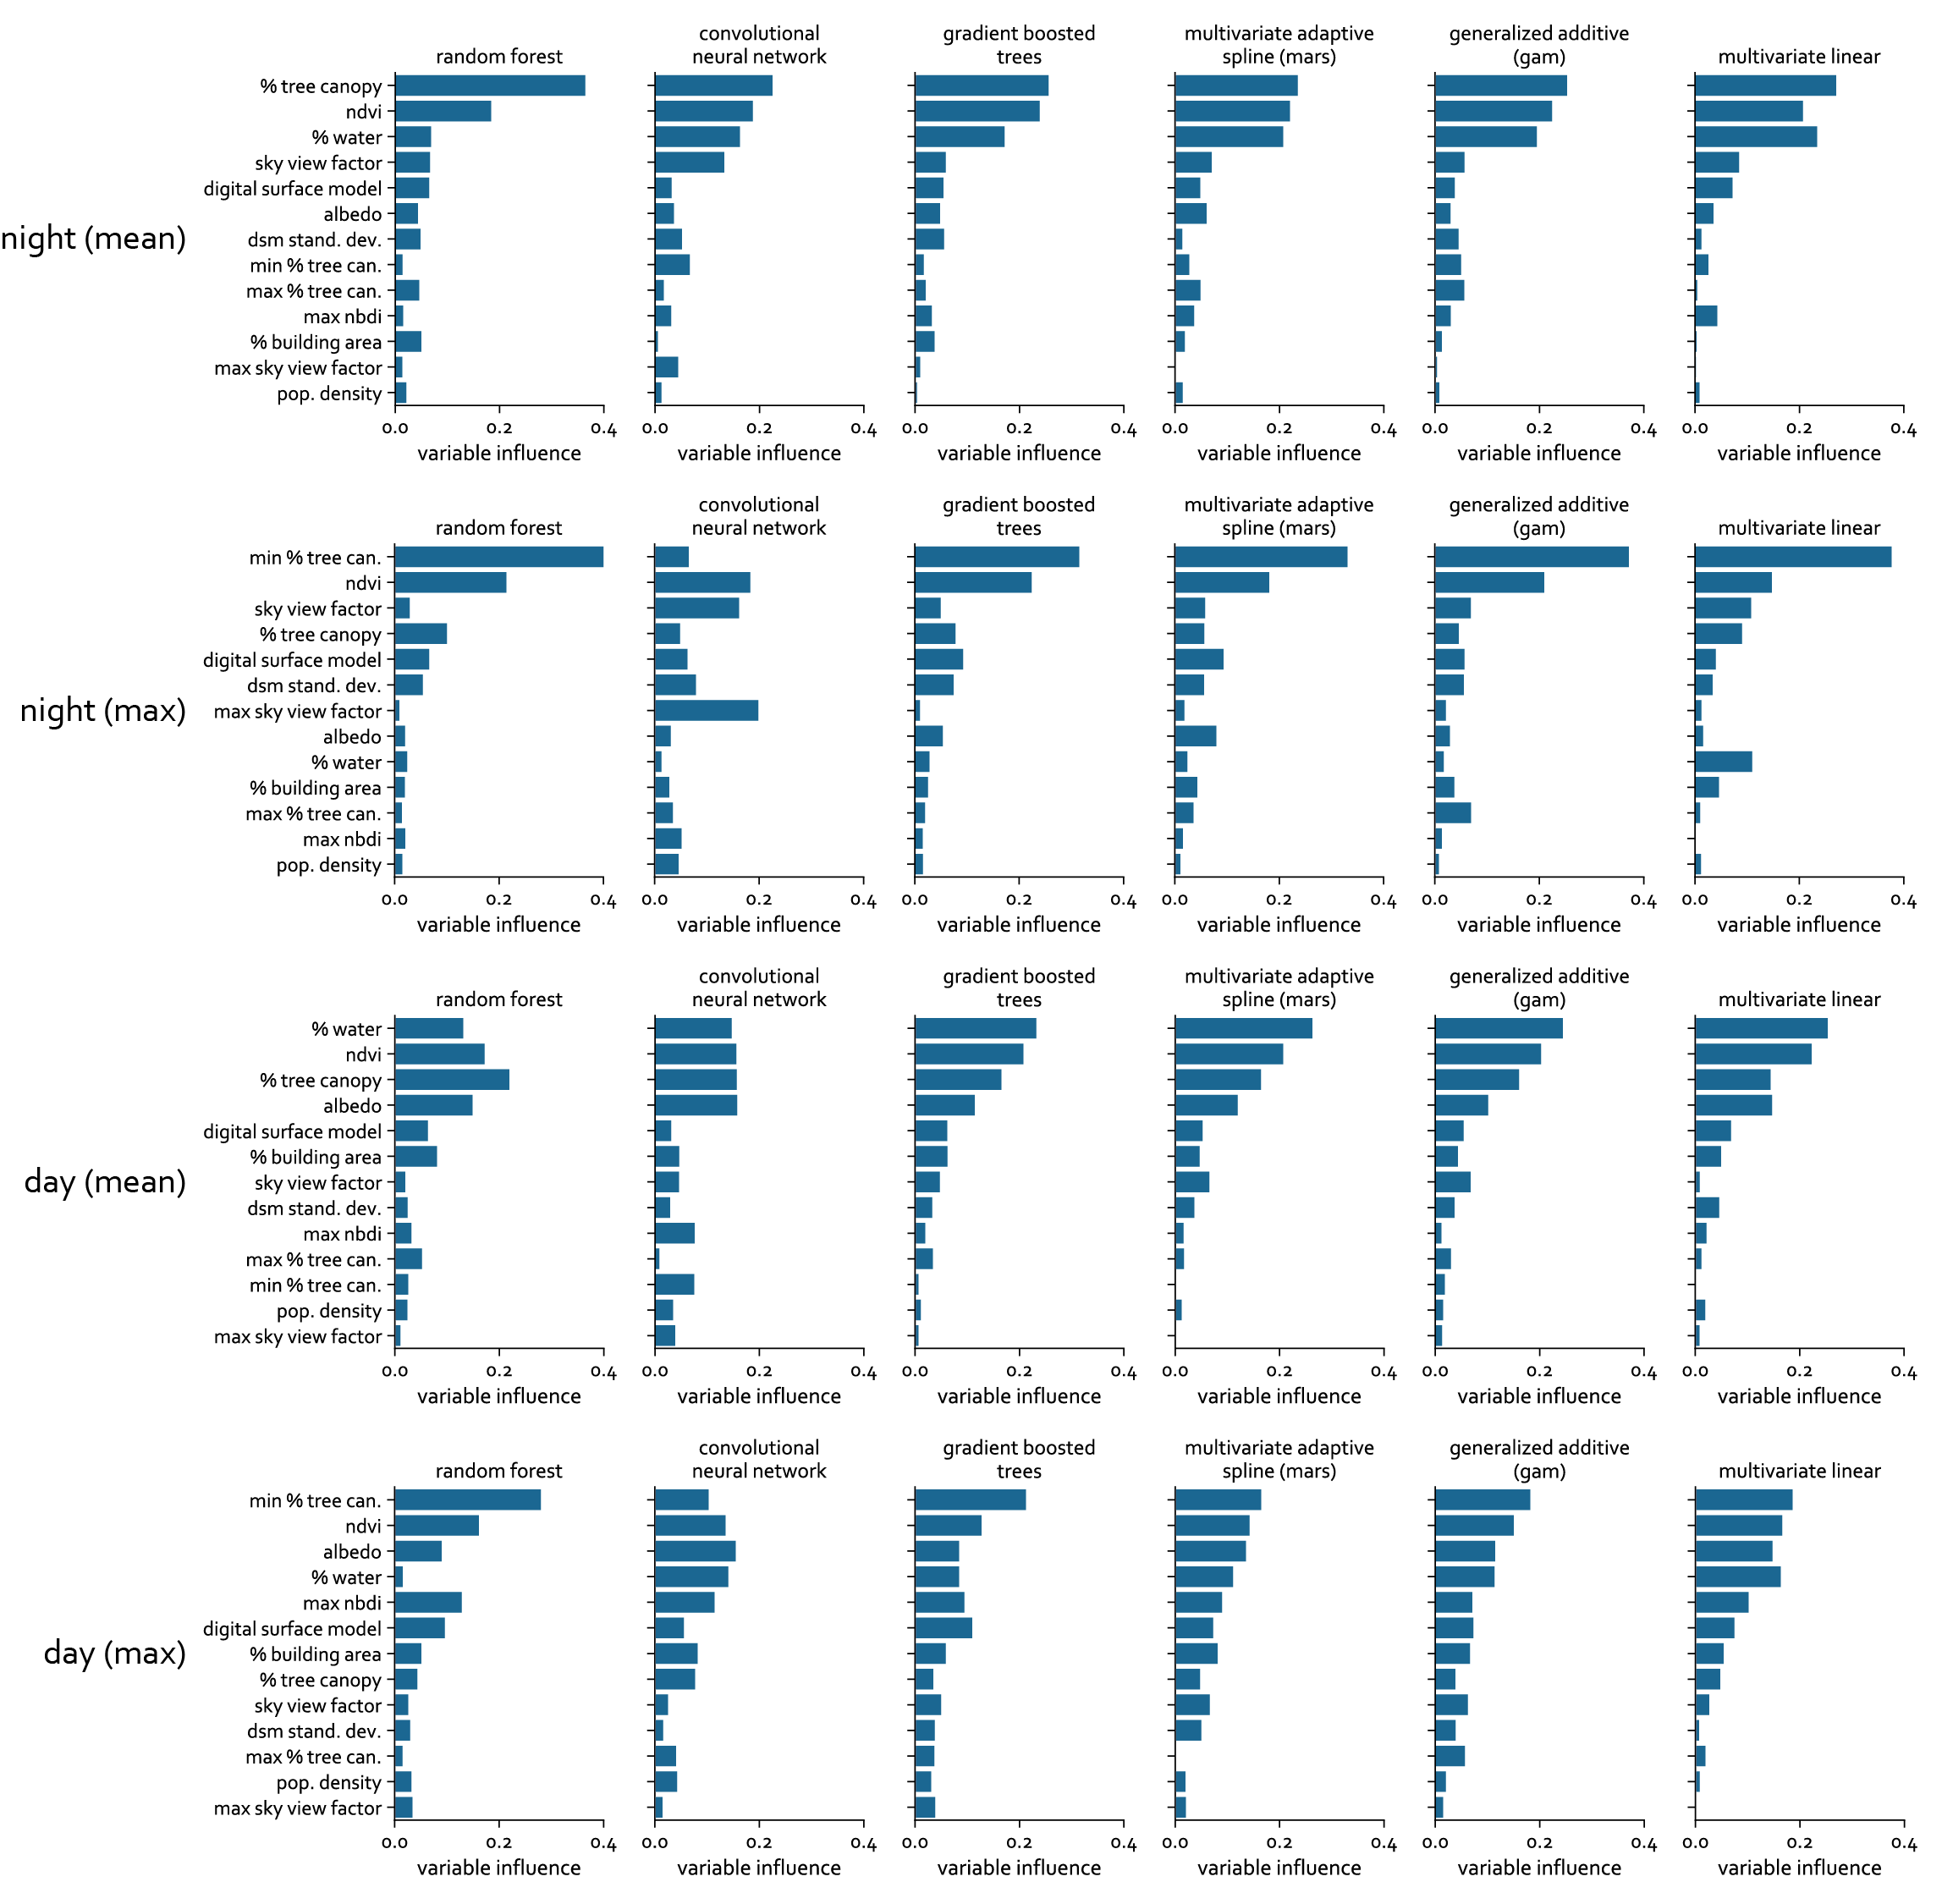
\includegraphics[width=\linewidth]{fig/report/importance_500.png}
    \caption[Variable influence on LST at 500-meter resolution]{
    Variable influence on LST at 500-meter resolution.
    The variable influence, measured by swing, shows the relative importance of each urban characteristic on land surface temperature.}
    \label{fig:importance_500}
    \end{center}
\end{figure*}


\clearpage
\section{City specific results}
\label{ss:city}
\begin{figure}[h]
    \centering
    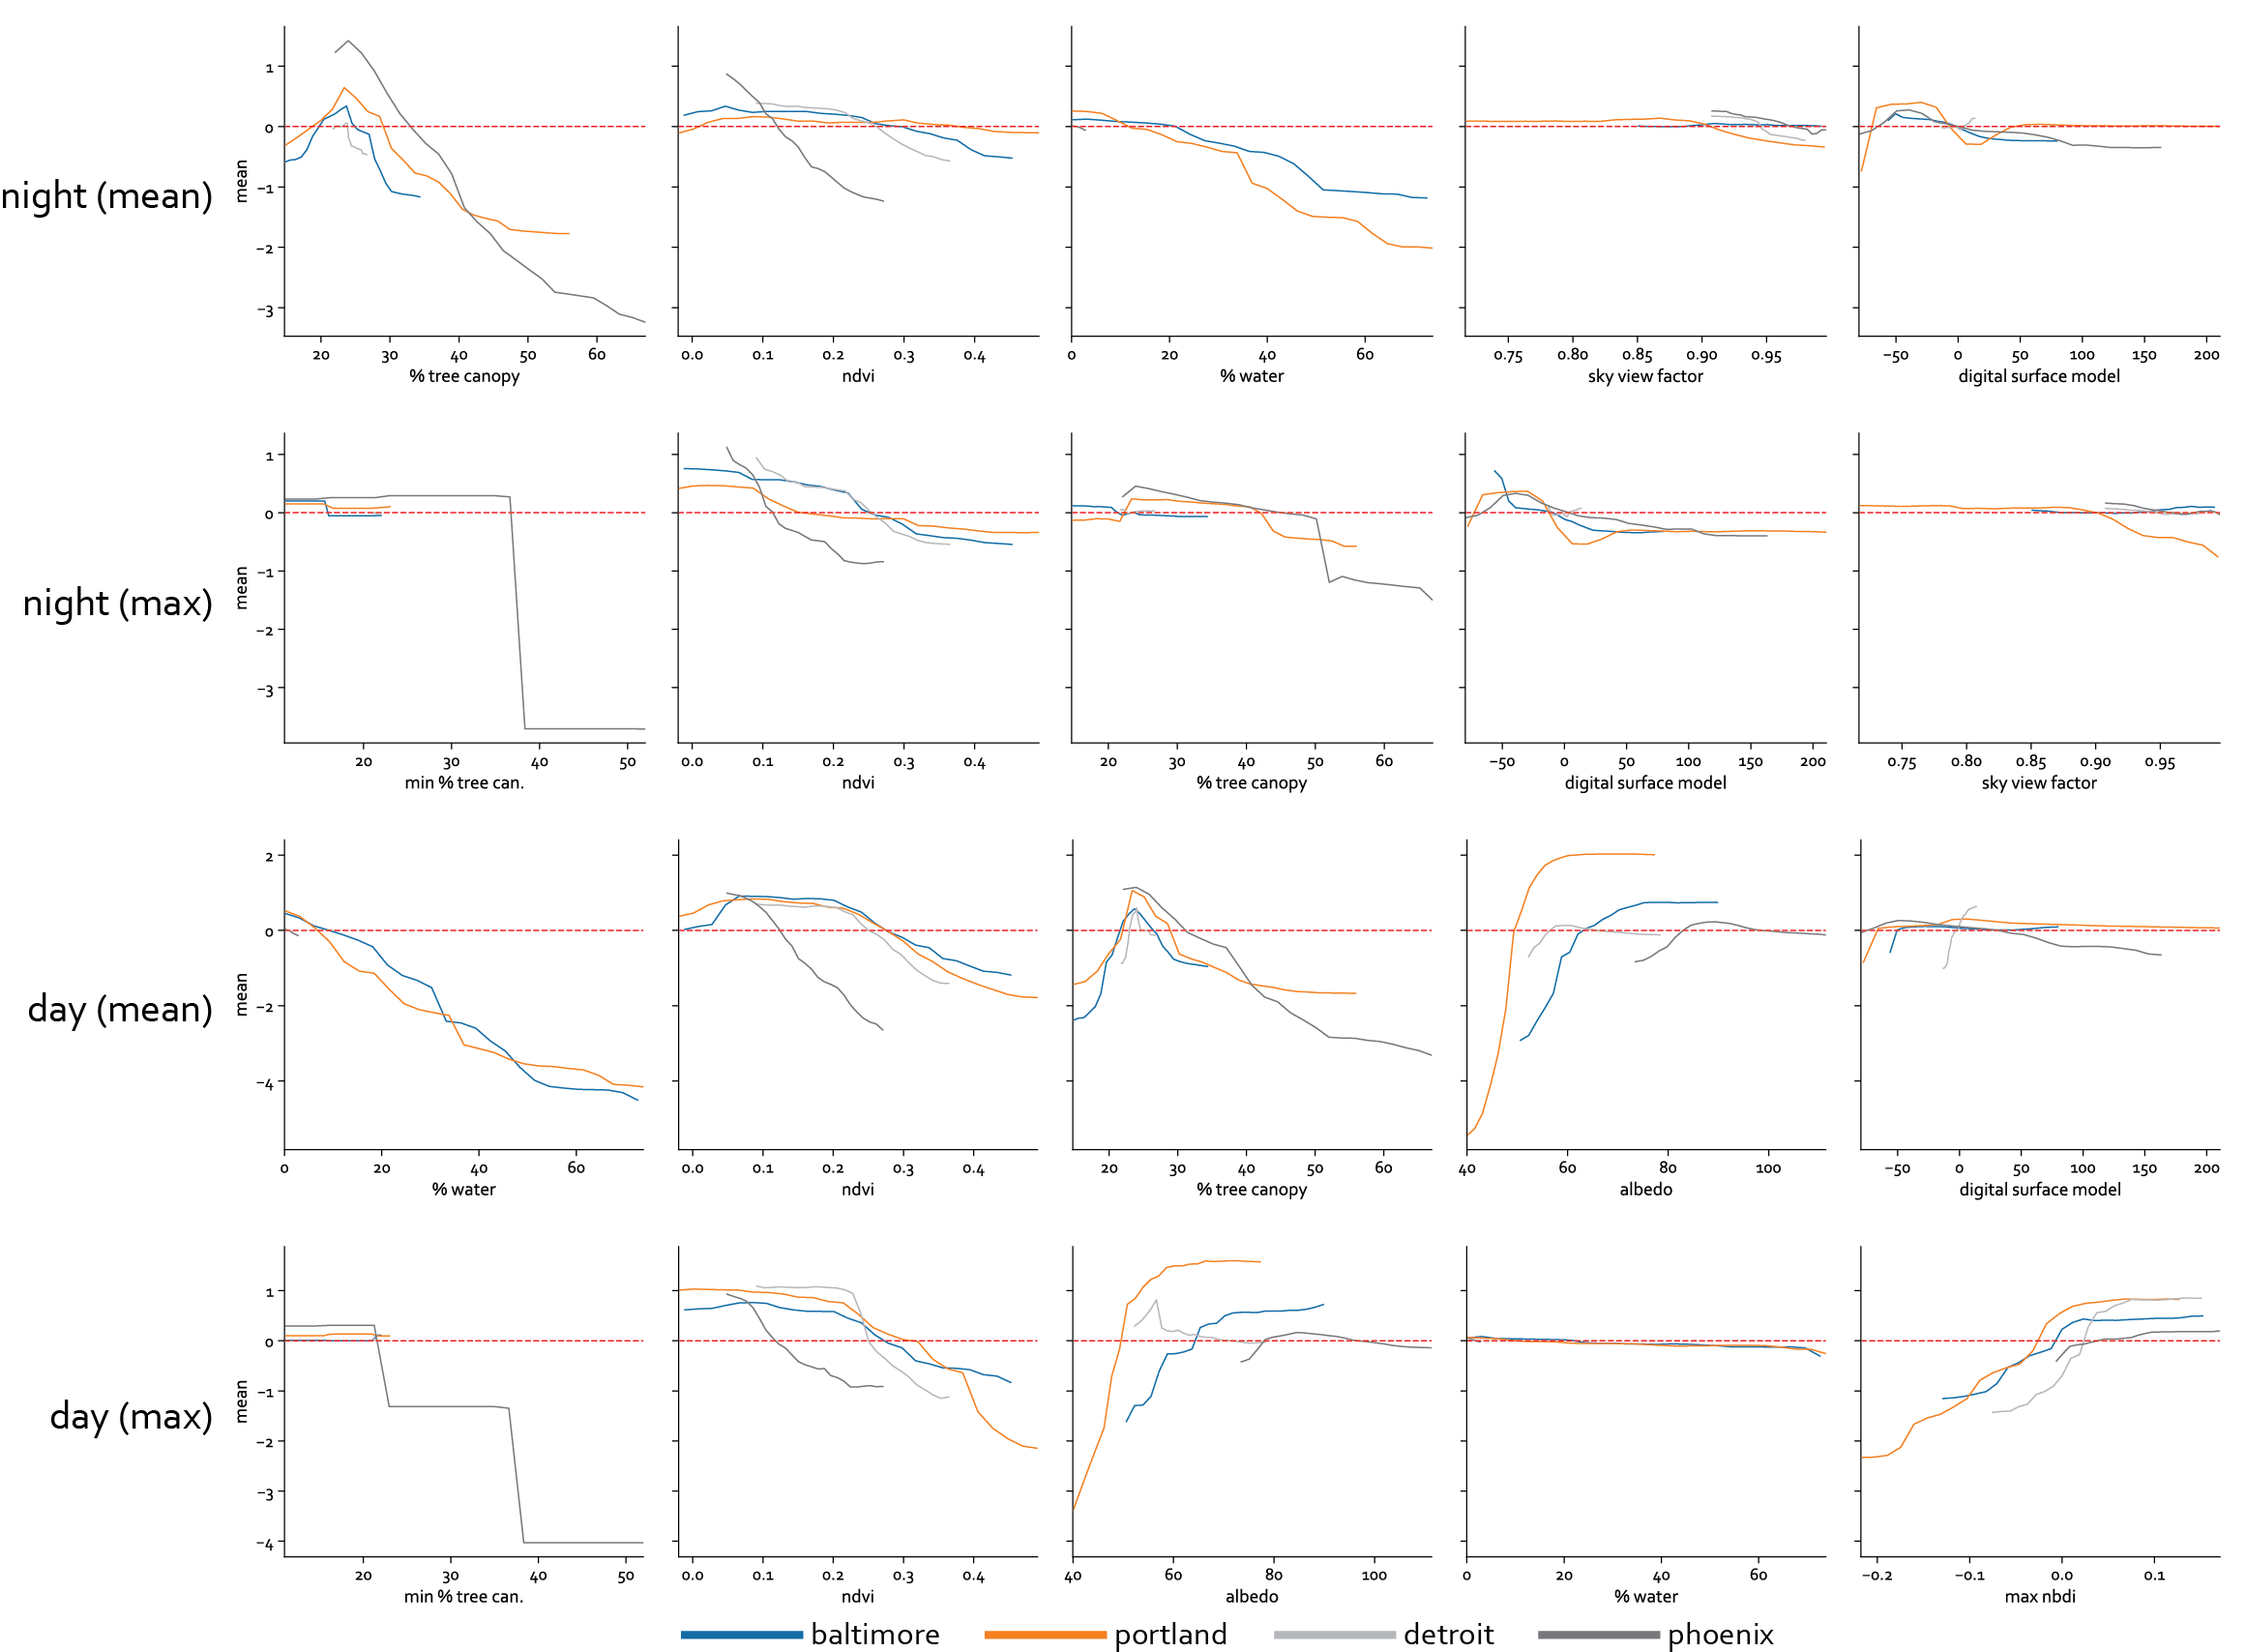
\includegraphics[width=\linewidth]{fig/report/pdp_cities_500.png}
    \caption[City specific partial dependence plots at the 500-meter resolution]{
    City specific partial dependence plots at the 500-meter resolution.
    The partial dependence plots for a random forest model trained on each city.
    This is to evaluate whether the influence of urban characteristics on LST is consistent between the cities.
    }
    \label{fig:cities_500}
\end{figure}

\begin{figure}[h]
    \centering
    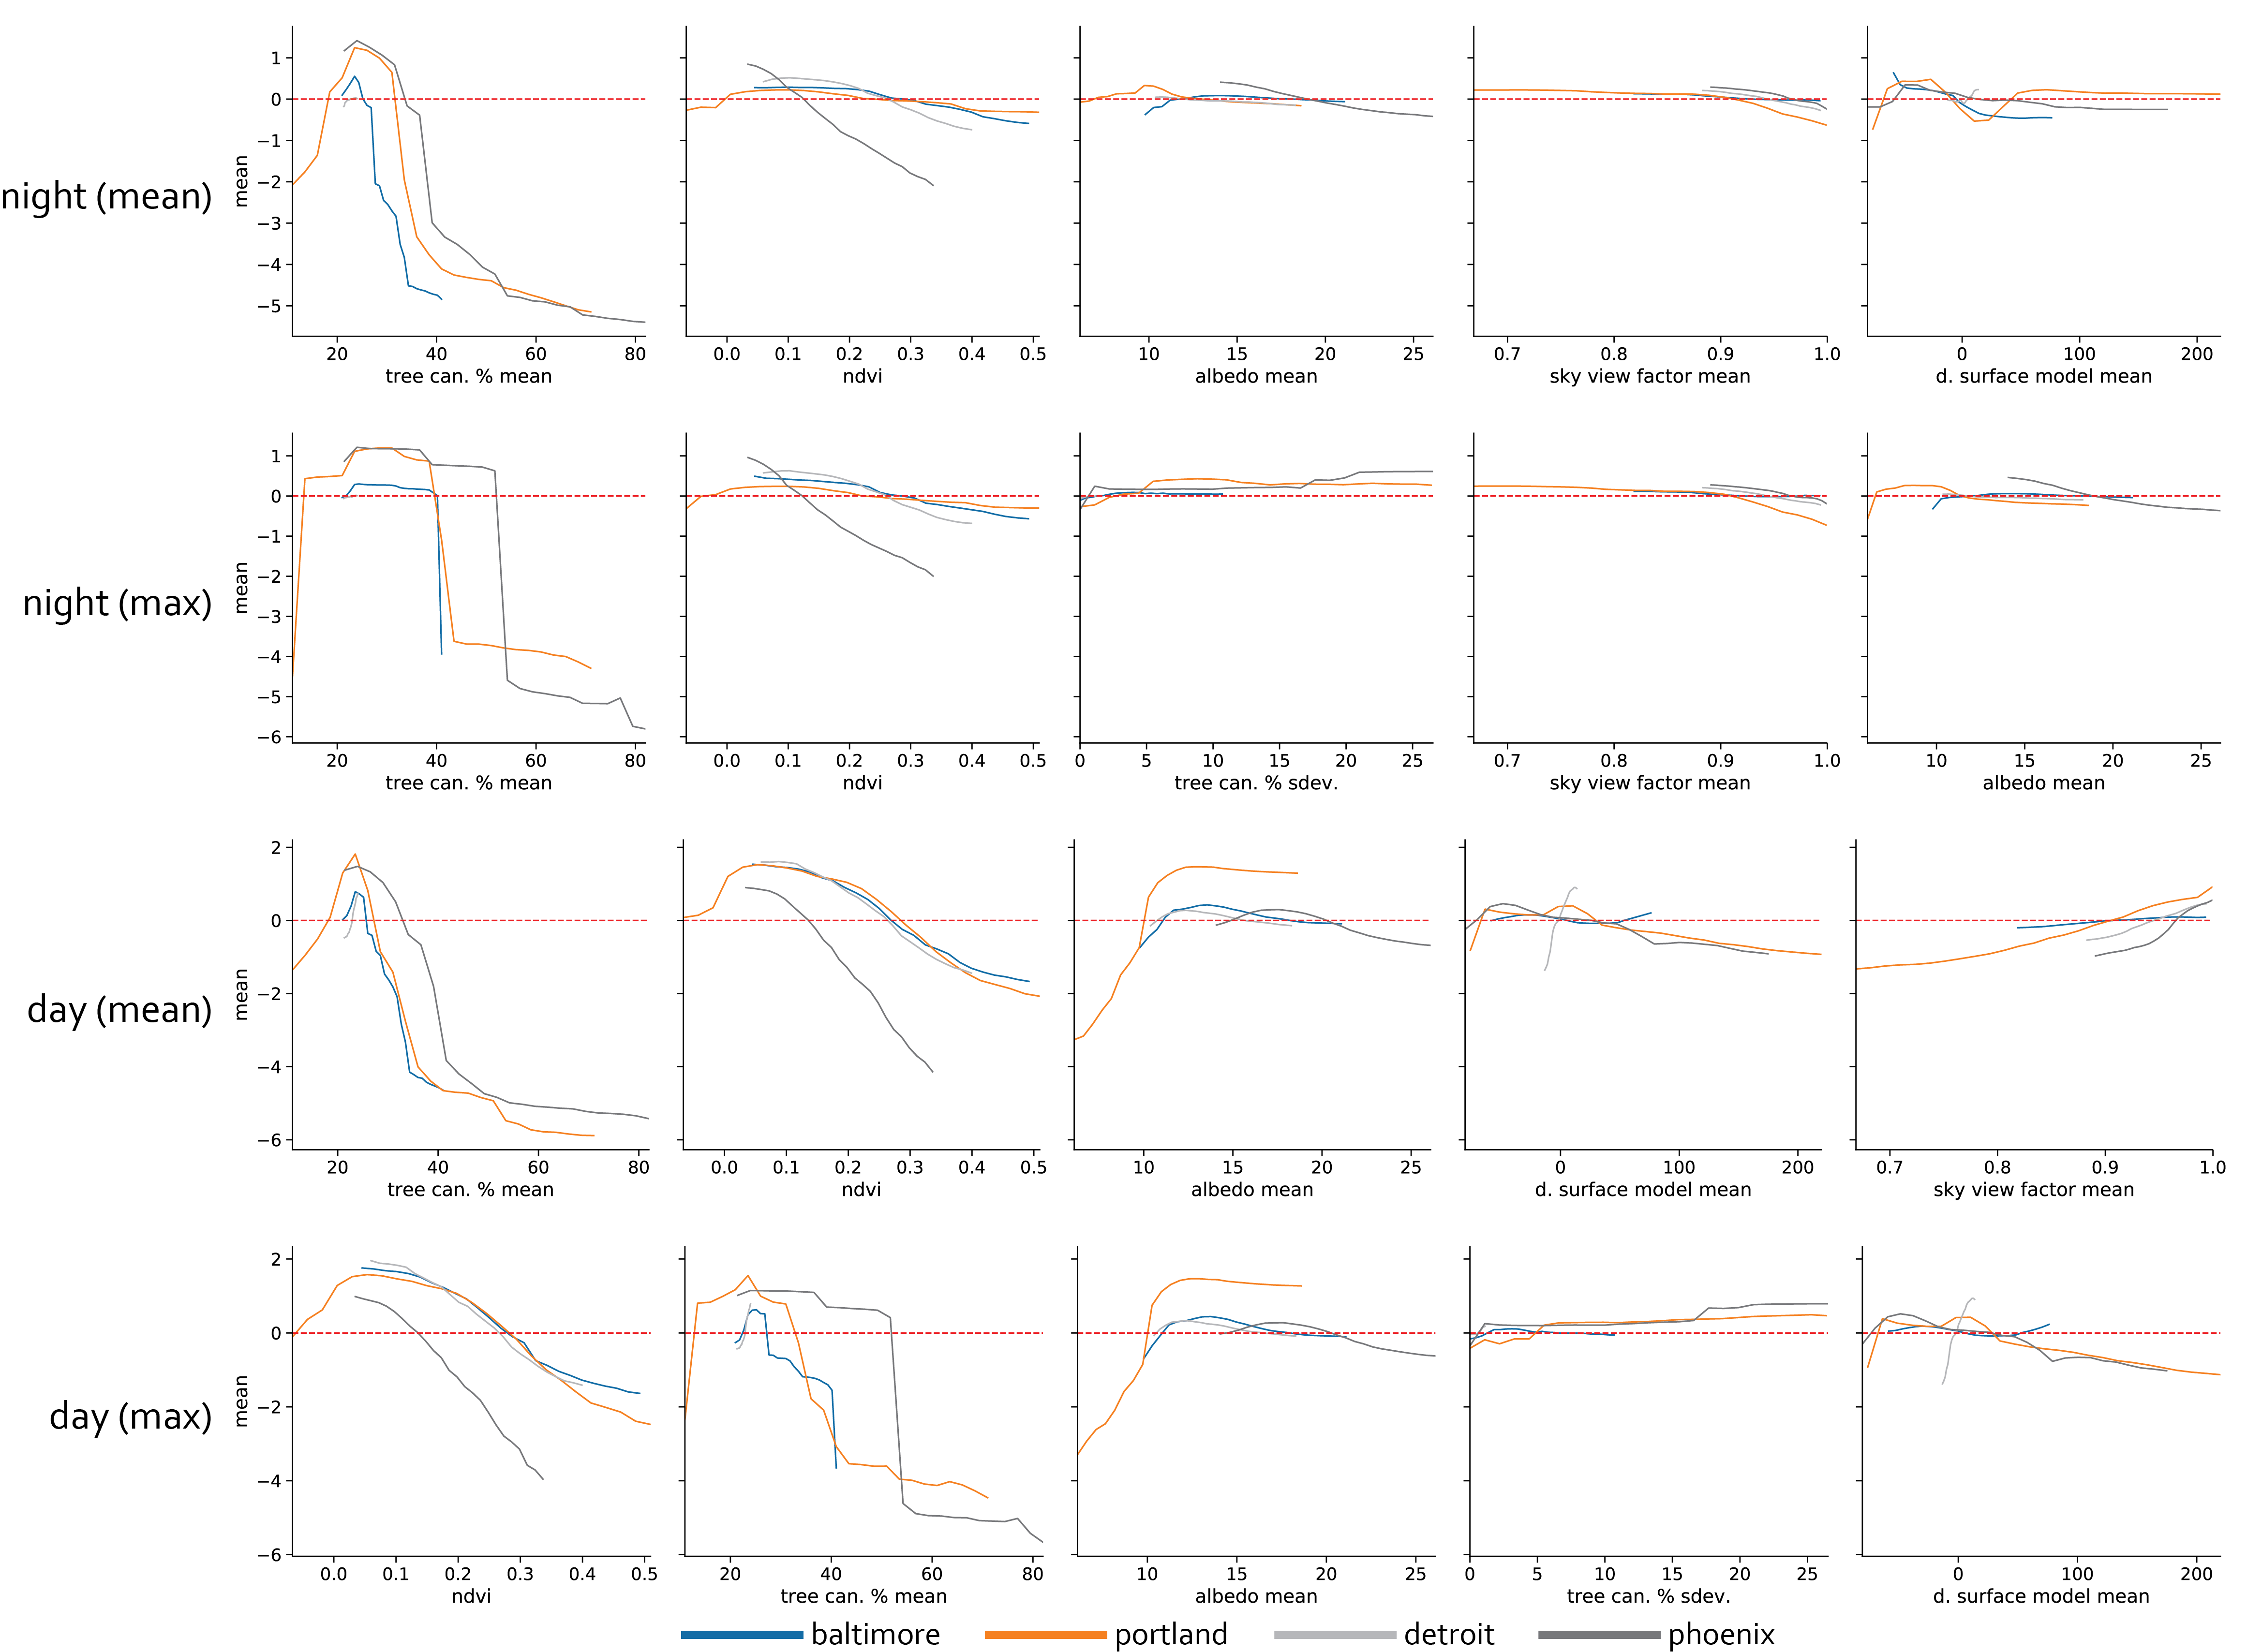
\includegraphics[width=\linewidth]{fig/report/pdp_cities_100.png}
    \caption[City specific partial dependence plots at the 100-meter resolution]{
    City specific partial dependence plots at the 100-meter resolution.
    These are partial dependence plots for a random forest model trained on each city.
    This is to evaluate whether the influence of urban characteristics on LST is consistent between the cities.
    }
    \label{fig:cities_100}
\end{figure}


\clearpage
\section{500-meter resolution results}
\label{ss:500_meter}
The figures presented in the main text, are replicated here based on data at a 500-meter resolution.

\begin{figure*}[h]
    \centering
    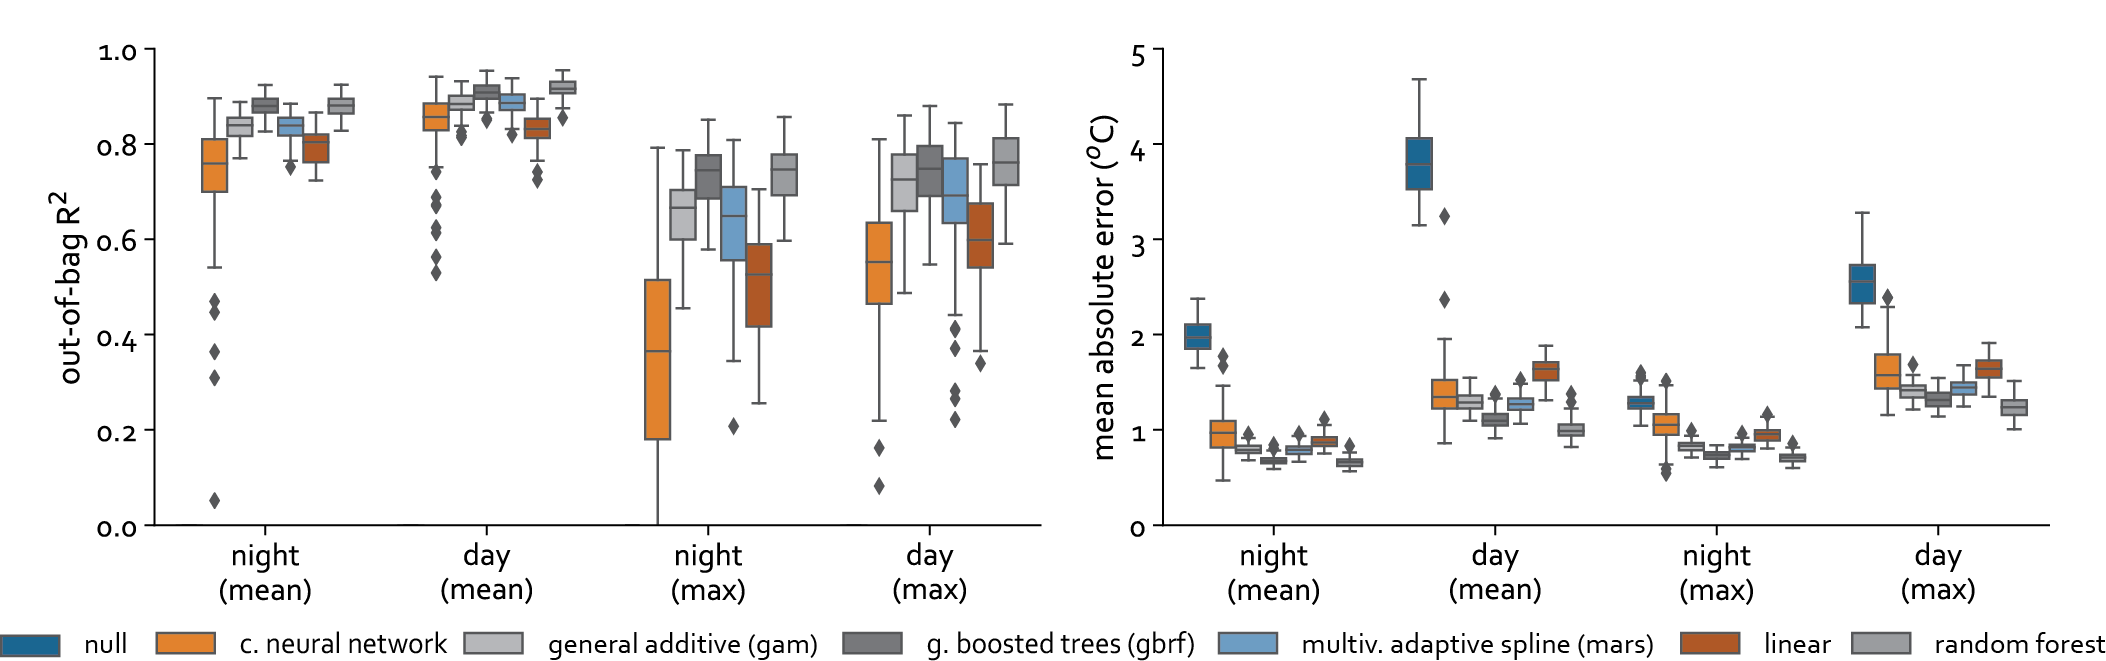
\includegraphics[width=\linewidth]{fig/report/holdout_500.png}
    \caption[Holdout cross-validation results at 500-meter resolution]{
    Holdout cross-validation results at 500-meter resolution. 
    The out-of-bag (OOB) R$^2$ and mean absolute error (MAE) of the models from a 500-fold holdout cross-validation. 
    The models were trained on 80\% of the data and tested on the unseen 20\%.
    When selecting data for the training and testing sets, spatial subsets were used to account for spatial similarities. 
    OOB R$^2$ can vary between $(-\infty, 1)$, where better models have a value near 1. 
    Good models have MAE near 0.
    }
    \label{fig:holdout_500}
\end{figure*}






\begin{figure*}[h]
    \centering
    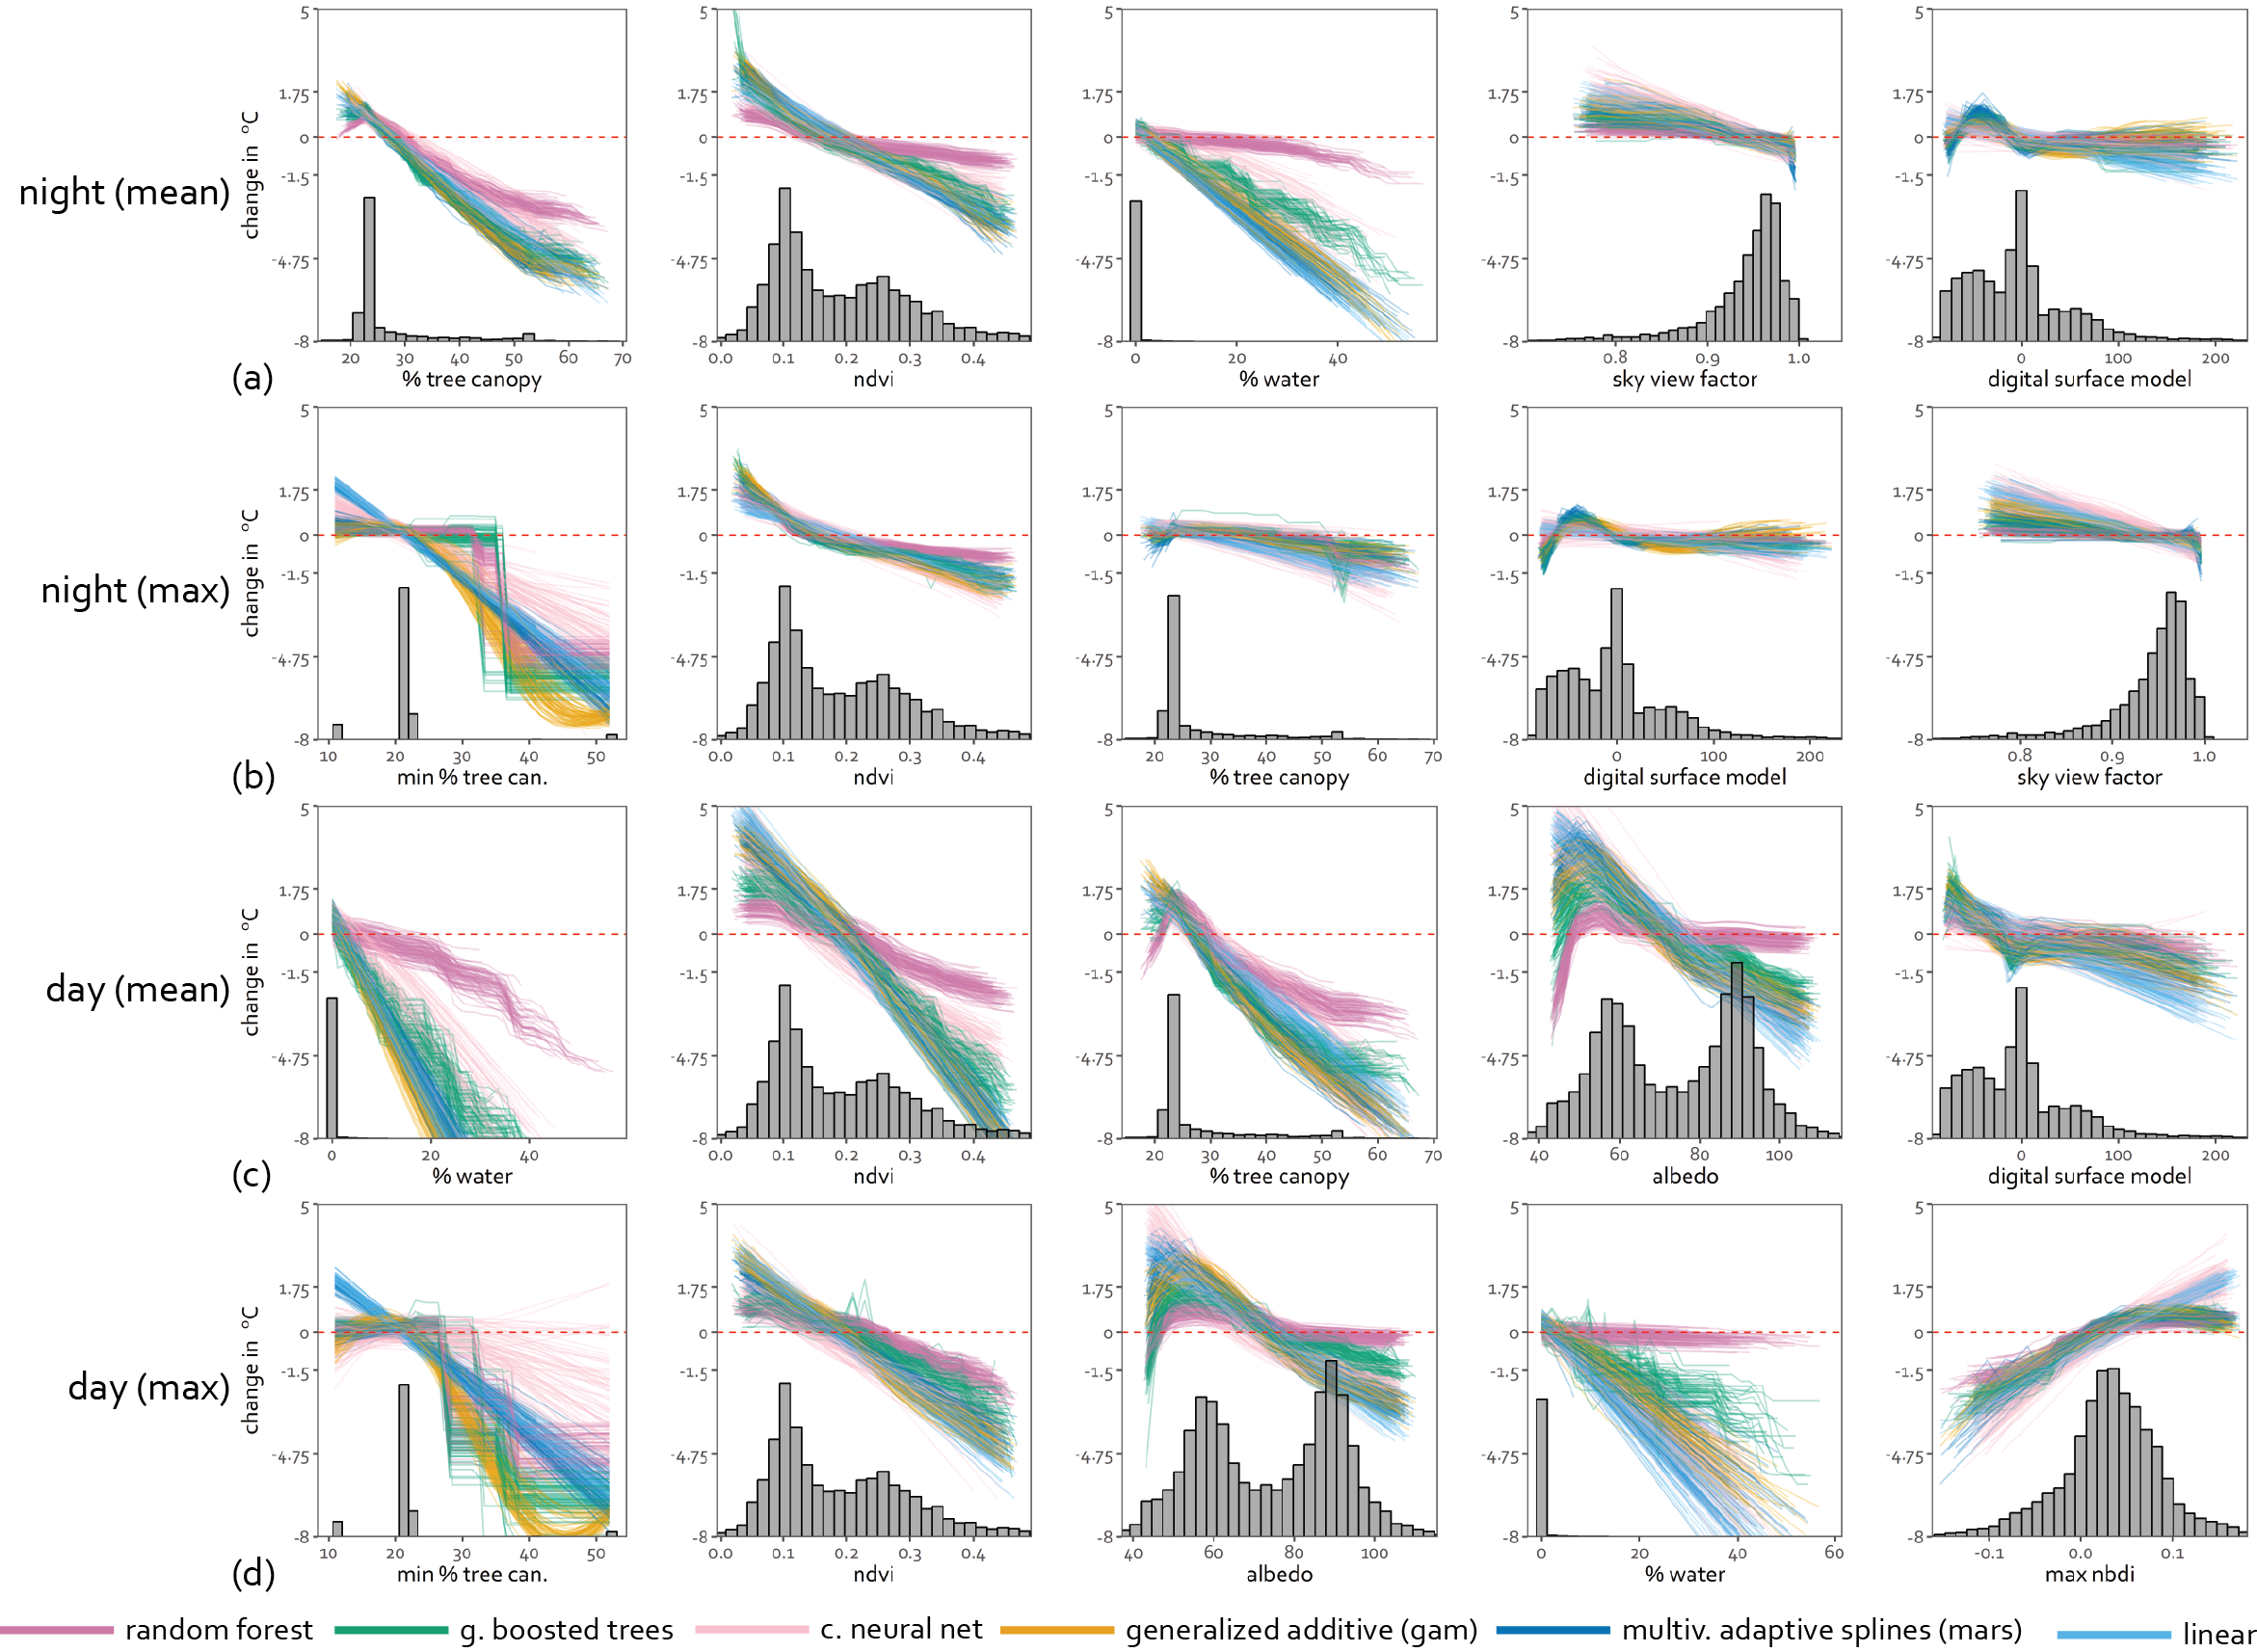
\includegraphics[width=\linewidth]{fig/report/pdp_500.png}
    \caption[Partial dependence plots for LST at 500-meter resolution]{
    Partial dependence plots for LST at 500-meter resolution.
    Partial dependence plots show how the land surface temperature ($^oC$, y axis) changes with each urban characteristic as the other variables are held at their average (mean) value. 
    The left hand side shows the effect each variable has on the (a) mean land surface temperature (LST) during the night, (b) maximum LST during the night, (c) mean LST during the day, (d) maximum LST during the day. 
    Each of the models are shown and this indicates the model uncertainty in the relationships.
    There are multiple lines for each model based on bootstrap samples of the data, which indicates the data uncertainty.
    The histograms on the $x$-axis shown the distribution of the observed data.
    }
    \label{fig:pdp_500}
\end{figure*}

\begin{figure}[h]
    \centering
    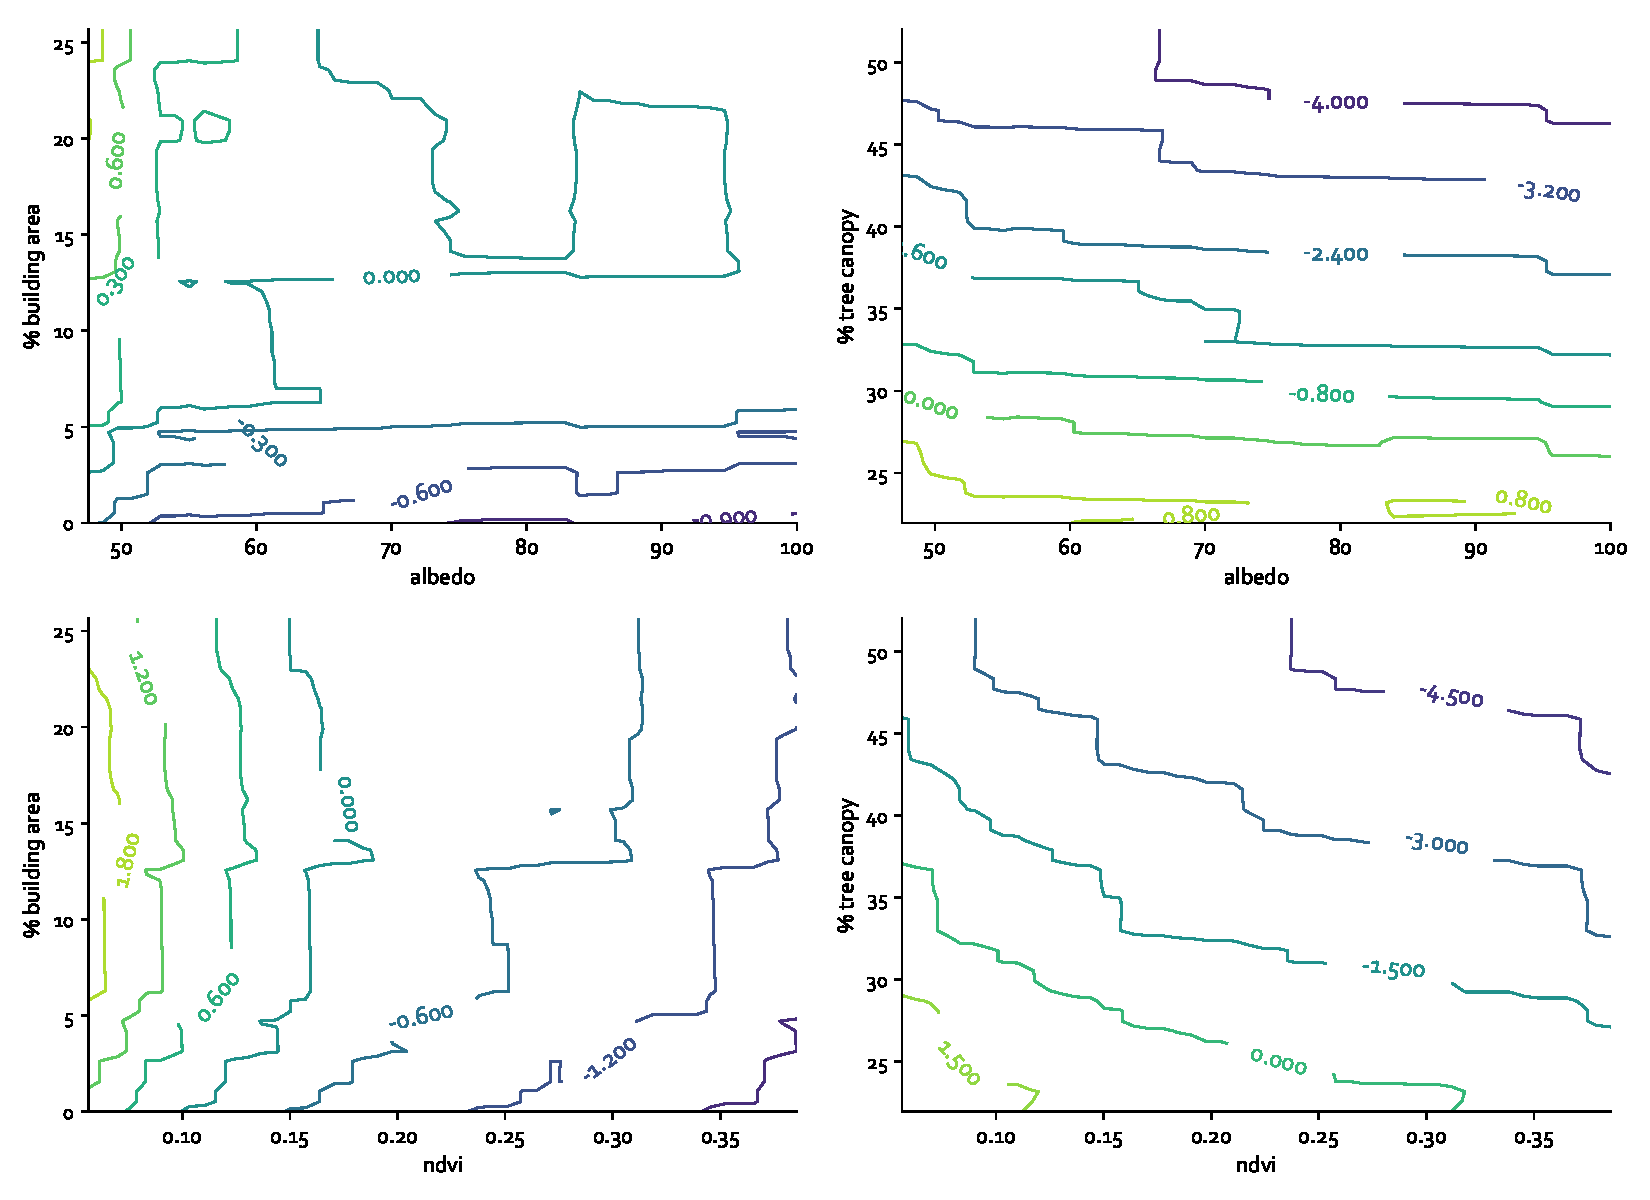
\includegraphics[width=\linewidth]{fig/report/pdp_2d_night_500.pdf}
    \caption[Partial dependence contour plots for LST at 500-meter resolution during the night]{
    \textbf{Night.} Partial dependence contour plots for LST at 500-meter resolution during the night.
    These partial dependence contours show how the land surface temperature ($^oC$, y axis) changes with each variable as the other variables are held at their average value.
    }
    \label{fig:pdp_2dnight_500}
\end{figure}

\begin{figure}[h]
    \centering
    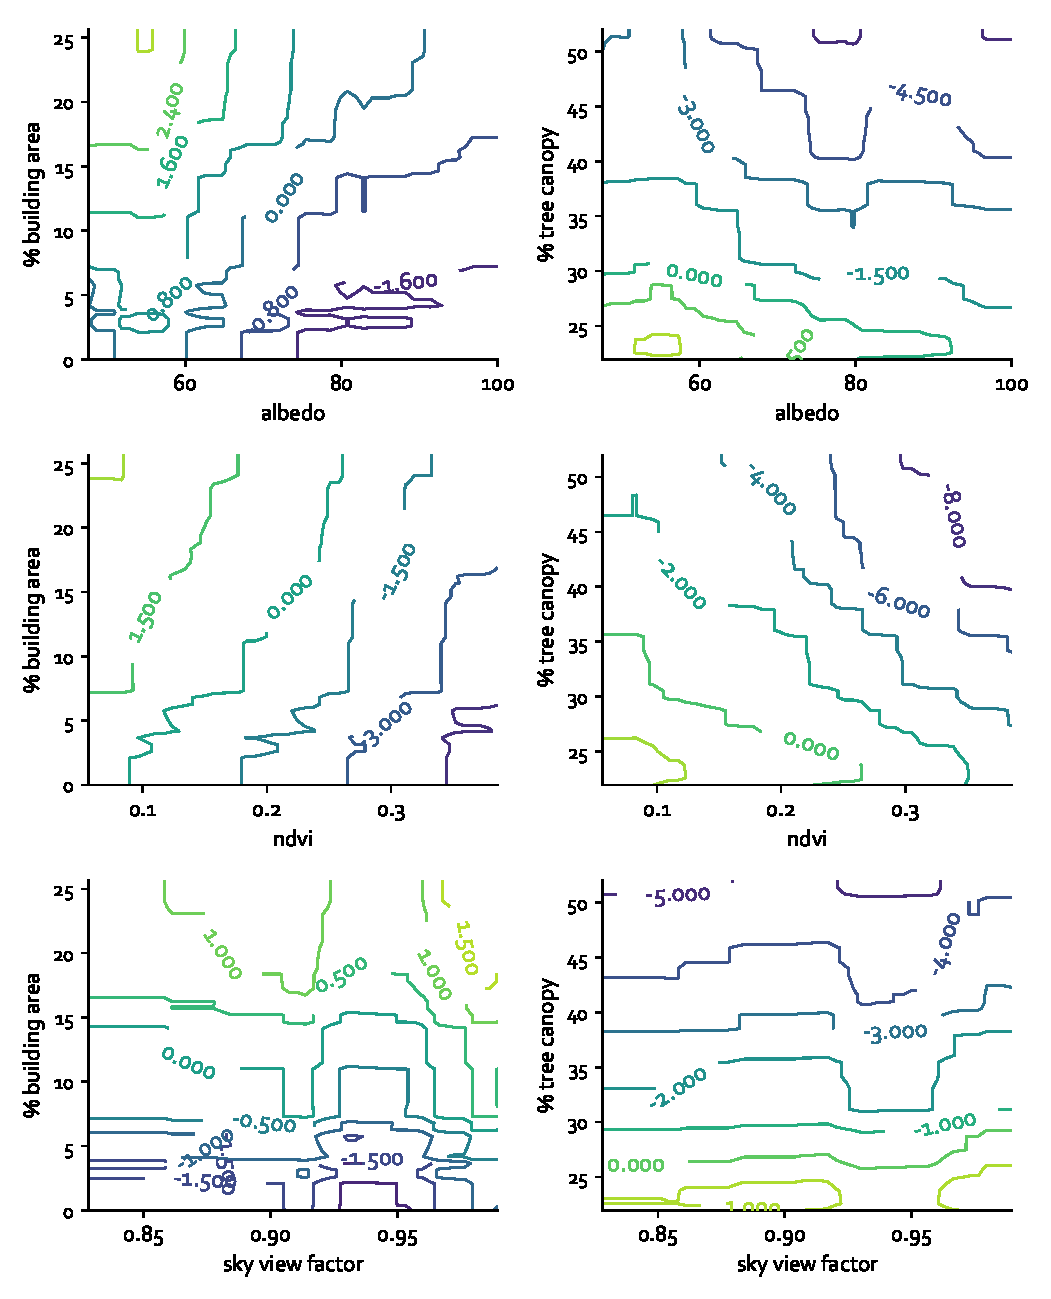
\includegraphics[width=\linewidth]{fig/report/pdp_2d_day_500.pdf}
    \caption[Partial dependence contour plots for LST at 500-meter resolution during the day]{
    \textbf{Day.} Partial dependence contour plots for LST at 500-meter resolution during the day.
    These partial dependence contours show how the land surface temperature ($^oC$, y axis) changes with each variable as the other variables are held at their average value. 
    }
    \label{fig:pdp_2dday_500}
\end{figure}


\clearpage
\section{Additional figures}
\begin{figure*}[h]
    \centering
    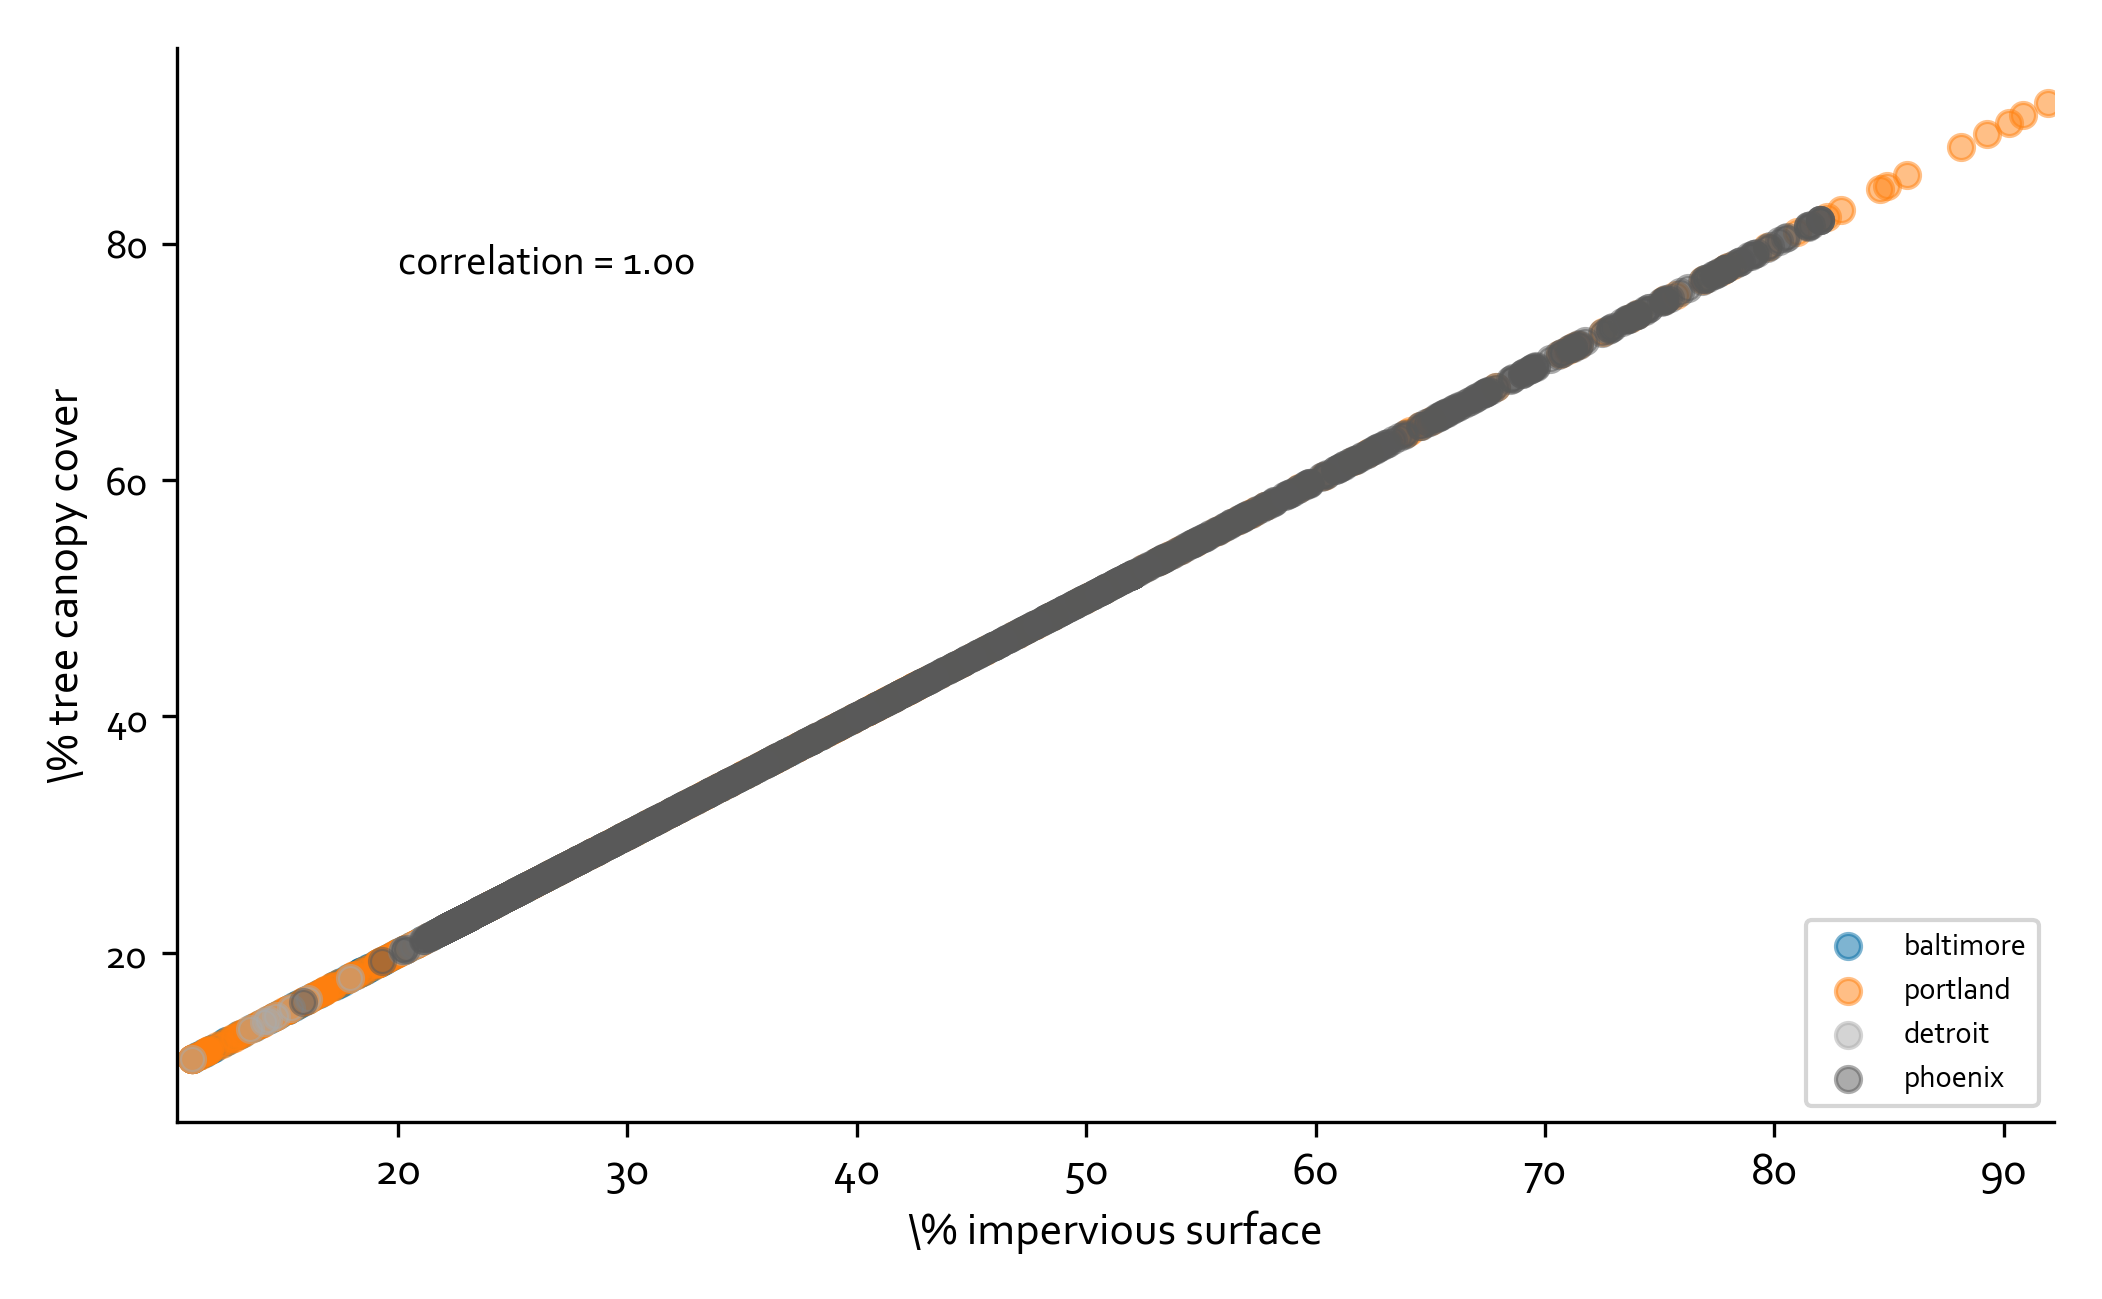
\includegraphics[width=\linewidth]{fig/report/imp_v_tree_500.png}
    \caption{
    In the MRLC data provided by the USA's National Land Cover Database, the percentage tree canopy cover and impervious surface are 100\% correlated. Therefore we can only use one of these two variables in our statistical models. In the results we discuss the two factors together.
    }
    \label{fig:imp_tree}
\end{figure*}


\end{document}
